\documentclass[twoside,leqno,twocolumn]{article}\usepackage[]{graphicx}\usepackage[]{color}
%% maxwidth is the original width if it is less than linewidth
%% otherwise use linewidth (to make sure the graphics do not exceed the margin)
\makeatletter
\def\maxwidth{ %
  \ifdim\Gin@nat@width>\linewidth
    \linewidth
  \else
    \Gin@nat@width
  \fi
}
\makeatother

\definecolor{fgcolor}{rgb}{0.345, 0.345, 0.345}
\newcommand{\hlnum}[1]{\textcolor[rgb]{0.686,0.059,0.569}{#1}}%
\newcommand{\hlstr}[1]{\textcolor[rgb]{0.192,0.494,0.8}{#1}}%
\newcommand{\hlcom}[1]{\textcolor[rgb]{0.678,0.584,0.686}{\textit{#1}}}%
\newcommand{\hlopt}[1]{\textcolor[rgb]{0,0,0}{#1}}%
\newcommand{\hlstd}[1]{\textcolor[rgb]{0.345,0.345,0.345}{#1}}%
\newcommand{\hlkwa}[1]{\textcolor[rgb]{0.161,0.373,0.58}{\textbf{#1}}}%
\newcommand{\hlkwb}[1]{\textcolor[rgb]{0.69,0.353,0.396}{#1}}%
\newcommand{\hlkwc}[1]{\textcolor[rgb]{0.333,0.667,0.333}{#1}}%
\newcommand{\hlkwd}[1]{\textcolor[rgb]{0.737,0.353,0.396}{\textbf{#1}}}%
\let\hlipl\hlkwb

\usepackage{framed}
\makeatletter
\newenvironment{kframe}{%
 \def\at@end@of@kframe{}%
 \ifinner\ifhmode%
  \def\at@end@of@kframe{\end{minipage}}%
  \begin{minipage}{\columnwidth}%
 \fi\fi%
 \def\FrameCommand##1{\hskip\@totalleftmargin \hskip-\fboxsep
 \colorbox{shadecolor}{##1}\hskip-\fboxsep
     % There is no \\@totalrightmargin, so:
     \hskip-\linewidth \hskip-\@totalleftmargin \hskip\columnwidth}%
 \MakeFramed {\advance\hsize-\width
   \@totalleftmargin\z@ \linewidth\hsize
   \@setminipage}}%
 {\par\unskip\endMakeFramed%
 \at@end@of@kframe}
\makeatother

\definecolor{shadecolor}{rgb}{.97, .97, .97}
\definecolor{messagecolor}{rgb}{0, 0, 0}
\definecolor{warningcolor}{rgb}{1, 0, 1}
\definecolor{errorcolor}{rgb}{1, 0, 0}
\newenvironment{knitrout}{}{} % an empty environment to be redefined in TeX

\usepackage{alltt}

\newcommand{\algoname}{\textsc{BenFound}}
\newcommand{\eDiv}{\textsc{eDiv}}
\newcommand{\eAgglo}{\textsc{eAgglo}}
\newcommand{\cpppo}{\textsc{cp3o}}
\newcommand{\pDPA}{\textsc{pDPA}}
\newcommand{\TED}{\textsc{TED}}
\newcommand{\BinSegMean}{\textsc{BinSeg-Mean}}
\newcommand{\BinSeg}{\textsc{BinSeg}}
\newcommand{\BinSegVar}{\textsc{BinSeg-Var}}
\newcommand{\BinSegMeanVar}{\textsc{BinSeg-MeanVar}}

\usepackage{ltexpprt}

\usepackage{amsfonts}
\IfFileExists{upquote.sty}{\usepackage{upquote}}{}
\begin{document}




% \setcounter{chapter}{2} % If you are doing your chapter as chapter one,
% \setcounter{section}{3} % comment these two lines out.

\title{Let's see your Digits: Anomalous-State Detection using Benford's Law}
\author{Samuel Maurus\thanks{Helmholtz Zentrum Munich, Technical University of Munich, samuel.maurus@helmholtz-muenchen.de} \\
  \and
  Claudia Plant\thanks{University of Vienna, claudia.plant@univie.ac.at}}
\date{}

\maketitle


% \pagenumbering{arabic}
% \setcounter{page}{1}%Leave this line commented out.

\begin{abstract} \small\baselineskip=9pt Benford's Law explains a curious ``naturally-occurring'' phenomenon in which the leading digits of numerical data are distributed in a precise fashion. In this paper we begin by showing that system metrics generated by many modern information systems like Twitter, Wikipedia, YouTube and GitHub obey this law. We then propose a novel unsupervised approach called \algoname{} that exploits this property to detect anomalous system events. \algoname{} tracks the ``Benfordness'' of key system metrics, like the follower counts of tweeting Twitter users or the change deltas in Wikipedia page edits. It then applies a novel Benford-conformity test in real-time to identify ``non-Benford events''. We investigate a variety of such events, showing that they correspond to unnatural and often undesired system interactions like spamming, hashtag-hijacking and denial-of-service attacks. The result is a technically-uncomplicated and effective  ``red flagging'' technique. Although not without its limitations, it is highly efficient and requires neither obscure parameters, text streams nor natural-language processing.\end{abstract}

\section{Introduction}
\label{sec:introduction}
% no \IEEEPARstart

In various domains it is useful to know if the interactions with a running system deviate from expected patterns. A canonical example is financial fraud, where organizations have an interest in exposing any persons attempting to deceive their funding and accounting processes. Other examples include online collaborative ecosystems like Twitter and Wikipedia, which strive to promptly detect and suppress behavior like spamming and attacks which can degrade service quality \cite{twitterTos}.

On the surface, such manipulative behavior may appear normal and be difficult to detect. A tax cheat may fabricate figures that, although dishonest, lie within expected ranges. Analogously, a spammer may use a team of fake Twitter accounts, each of which have sensible numbers of followers and friends. The manner in which the \textit{absolute values} of such numbers are distributed is often not unusual.

The key to the effectiveness of Benford's Law (BL) in such situations lies with its observation that the \textit{leading digits} of many sets of numbers are, by nature, distributed in a surprisingly \textit{non-uniform} way. In contrast, if such numbers are \textit{fabricated}, the leading digits rarely follow that same distribution. For example, the success of BL in financial auditing has shown that the na\"{\i}ve fraudster, in an attempt to contrive believable figures that are varied and ``well spread'', often fabricates figures with a more or less uniform distribution of leading digits \cite{nigrini2012}. When doing a Benford analysis, we focus \textit{only} on the leading digits and \textit{purposefully discard the magnitude information}. In this work we propose that monitoring the resulting digit distribution is a novel, robust and elegant mechanism for tracking the integrity of complex systems.



% Here we display the first histogram
\begin{knitrout}
\definecolor{shadecolor}{rgb}{0.969, 0.969, 0.969}\color{fgcolor}\begin{figure}[t!]
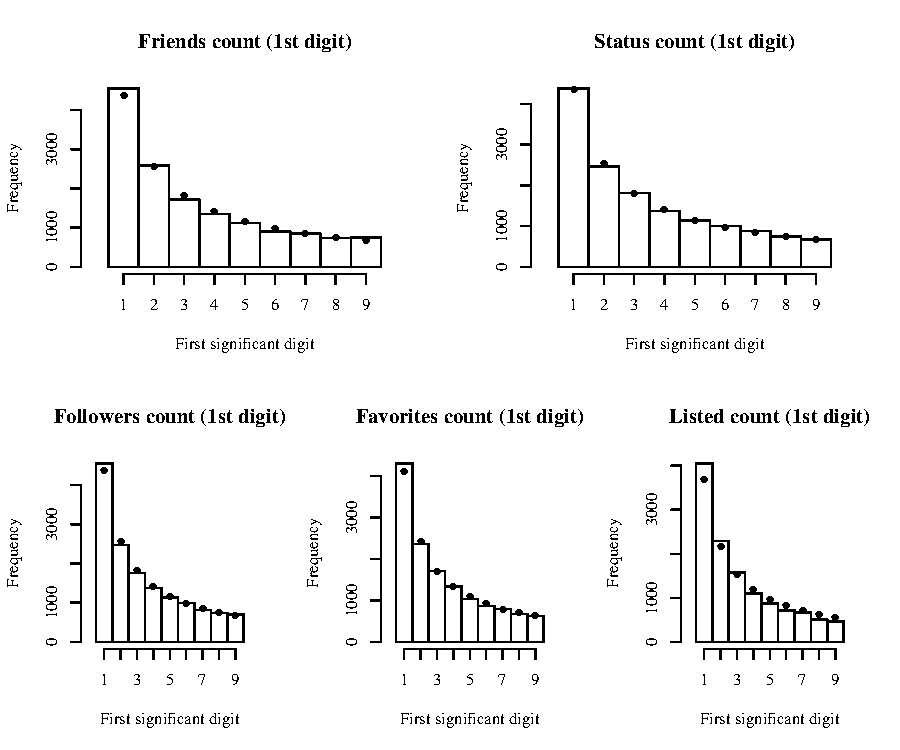
\includegraphics[width=\maxwidth]{figure/twitter-count-distributions-1} \caption[First-digit distributions for the five count-based metrics of 15,000 randomly-chosen Twitter users (friend-, status-, follower-, favorite- and listed-count)]{First-digit distributions for the five count-based metrics of 15,000 randomly-chosen Twitter users (friend-, status-, follower-, favorite- and listed-count). The bars represent the measured frequencies, and the filled bullets those predicted by Benford's Law.}\label{fig:twitter-count-distributions}
\end{figure}


\end{knitrout}

To grasp the basic concept of BL, we share measurements collected from 15,000 randomly-chosen Twitter users. If we consider the number of followers that each user has, we may see that one user has \textbf{2}93,845 followers while another has only \textbf{3}20. As an exercise in curiosity, how would we expect the distribution to appear when tallying just the first significant digit (marked in \textbf{bold}) of each value? That is, how likely is it that one of our 15,000 users has a follower-count that begins with the digit $9$ versus the digit $1$? To those unfamiliar with BL, the usual answer is ``equally likely''.

As Figure \ref{fig:twitter-count-distributions} shows, however, the distribution is far from uniform. Indeed, it defies intuition: it tells us that finding a follower-count starting with a $1$ is \textit{over six times more likely} than finding one starting with a $9$. This observation is not unique to this sample. In the same figure we see the distributions for the four other Twitter count-based metrics for each user (friend, listed, status, and favorited counts). All have the same basic form, and we can visually see a strong agreement with the BL predictions in each case. Considering that data from services such as Twitter are considered noisy \cite{antoine2015portraying, hayashi2015real}, this strong BL-conformity is a useful property.

% A note about the collection of the Twitter data. The raw data contains 14698 users with five measurements for each. In order, they are 1) friends_count, 2) statuses_count, 3) followers_count, 4) favorites_count and 5) listed_count.
% Note that we omit zero measurements for obvious reasons (they have no first significant digit)
% Data collection: we used the user-search feature of the Twitter API in March 2016. The search endpoint only allows a maximum of 1000 results returned and a search query is required. For this reason we used 15 of the most common trigraphs in the English language as the search terms: ["the", "and", "tha", "ent", "ion", "tio", "for", "nde", "has", "nce", "edt", "tis", "oft", "sth", "men"]. These were chosen based on the data presented on http://www.rollingr.net/wordpress/2007/02/02/common-letter-sequence/. For each search term (trigraph), we harvested the five metrics from the 1000 users returned from the endpoint. 
% Although we concede that this is not the most ideal random-sampling strategy, we argue that it is reasonable given the constraints of the Twitter API. We are confident that any other sensible sampling technique would yield very similar results (with respect to obeying bBenford's law).

In this paper we exploit the BL-conformity of such systems to form an intriguing foundation for describing what it means for systems to be in their ``expected'' or  ``natural'' state. We then present an approach for the detection of ``unexpected'' or  ``unnatural'' deviations from that state. Just as Benford's Law can expose fraudulent behavior in financial reports not seen by other tools, we show that the events detected by our framework are not found by state-of-the-art anomaly- and event-detection techniques. \newline

\noindent \textbf{Contributions:}

\noindent\textbf{1) We show the Benfordness of key metrics} tracked by Twitter, Wikipedia, YouTube and GitHub (Sections \ref{sec:introduction}, \ref{sec:case-study:-github} and \ref{sec:bot-detection-using-benfords-law}).

\noindent\textbf{2) We propose a test for Benford's Law conformity} exploiting the law's logarithmic basis and the formal Kolgomorov-Smirnov test (Section \ref{sec:test-conf-benf}).

\noindent\textbf{3) We present \algoname{} to detect ``unnatural'' events from streams of \textit{numerical data}}. \algoname{} does not require a text stream, nor any parameters other than the width $w$ of the sliding window (Section \ref{sec:extr-benf-sign}). It can be deployed in real-time and has linear run-time complexity in $w$.

\noindent\textbf{4) We present experiments on synthetic data}, showing that \algoname{} finds events not visible to state-of-the-art change-point and event-detection techniques that feed on numerical data (Section \ref{sec:synth-exper}).

\noindent\textbf{5) We present a number of real-world case-studies} showing how \algoname{} detects ``unnatural'' events not found by other techniques (Sections \ref{sec:bot-detection-using-benfords-law}, \ref{sec:case-study:-twitter}, \ref{sec:case-study:-outag}).


\section{Preliminaries}
\label{sec:preliminaries}

Benford's Law asserts that the probabilities for finding each of the nine possible digits $1,2,\ldots,9$ as the first significant digit are \textit{not equal}. It states that the digit 1, for example, occurs more than 30\% of the time and the digit 9 less than 5\% of the time. More precisely, given a vector $\vec{x} \in \mathbb{R}^n$ of numerical values, BL states that the probability of a randomly-selected element from $\vec{x}$ having the \textit{first} significant digit $d \in \{1,\ldots,9\}$ is

\begin{equation}
  \label{eq:bl-first-digit}
  P(D_1 = d) = \log_{10} (d+1) - \log_{10} (d).
\end{equation}

The bullets ($\bullet$) in Figure \ref{fig:twitter-count-distributions} were computed using these probabilities. The general form of BL further specifies the joint probability distribution of \textit{all} the significant digits \cite{berger2015Intro}\footnote{Note that the distributions for the second and higher digits quickly approach the uniform.}. 

Although it is clear that not \textit{all} sets of numbers obey the law (a sample of human heights in cm, for example, does not), Benford's original manuscript \cite{benford1938law} includes evidence supporting its wide application. Data from diverse sources as baseball statistics, death rates, lists of physical constants and randomly-selected numbers from newspapers were shown to conform. We recommend that the justifiably-skeptical reader perform a simple experiment in this light, such as randomly sampling numerical data from independent web pages.

Many familiar sequences follow BL. These include Fibonacci, the powers of (almost\footnote{For base ten it is clear that powers of any integer that is itself a power of ten (e.g. 1000) will not obey the law.}) any integer, and the factorials ($1!, \ldots, n!$). Such sequences offer an informal starting point for \textit{explaining} BL. It turns out that BL is often (but not always) observed to hold for sets of numbers spanning several orders of magnitude and associated with exponential or multiplicative growth processes. In this light, consider the sequence of numbers generated by the powers of 1.2 (that is, $1.2^1,1.2^2,1.2^3,\ldots$) plotted on a logarithmic axis:
\noindent
\begin{knitrout}
\definecolor{shadecolor}{rgb}{0.969, 0.969, 0.969}\color{fgcolor}
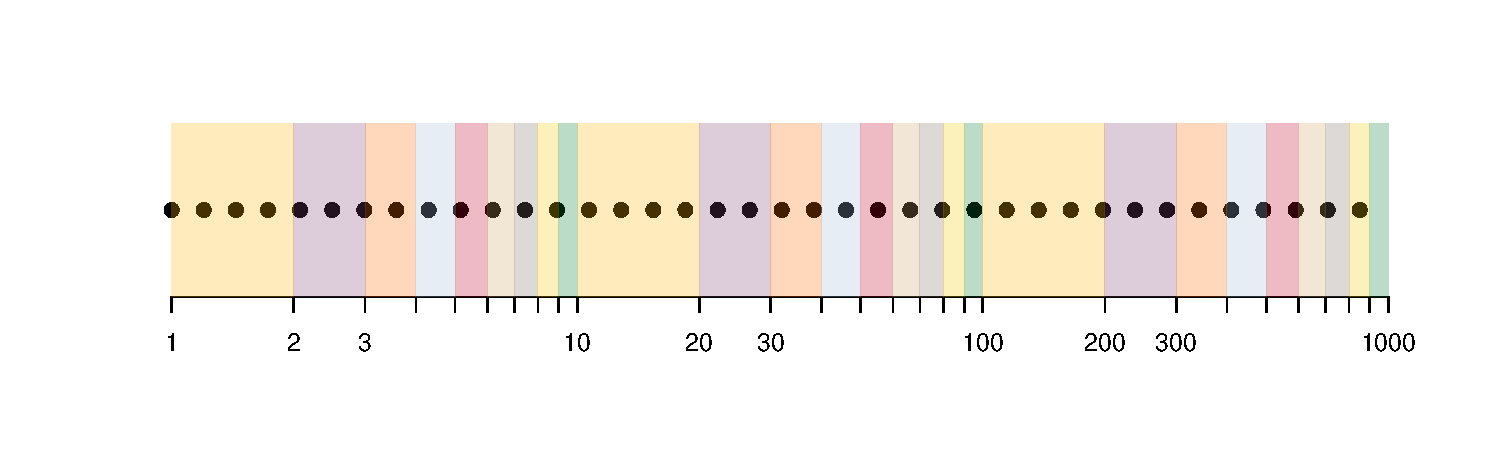
\includegraphics[width=\maxwidth]{figure/log-powers-of-two-1} 

\end{knitrout}

It is clear that the values are equally spread out when viewed on a logarithmic scale. It is then obvious that one of these values is more likely to fall into an interval where the first significant digit is one, that is, one of the intervals $[1,2)$, $[10,20)$, $[100,200)$ and so on. We can now understand the BL formula in Equation \ref{eq:bl-first-digit} graphically: the probability for any given digit is simply the width of its interval on the logarithmic scale.

With this in mind, let us consider the physiological and psychological reaction to external stimuli that we find in the real world. The growth of the sensation of brightness (Fechner's Law), the sense of loudness, the sense of weight, the response of the body to medicine or radiation, and the killing curves under toxins and radiation are all often logarithmic. In economics we often hear about percentage rates of growth. In social media, content can go ``viral'' with an exponentially growing number of views or downloads over time. As Benford himself elegantly noted: ``the analogy is complete, and one is tempted to think that the $1, 2, 3, \ldots$ scale is not the natural scale; but that, invoking the base $e$ of the natural logarithms, \textit{Nature} counts $e^0, e^x, e^{2x}, e^{3x}, \ldots$ and builds and functions accordingly'' \cite{benford1938law}.

Given that BL arises naturally, it should come as no surprise that it is base- and unit-invariant. This means that numbers obeying BL keep obeying BL after we express them in a different base (e.g. octal) or in different units (e.g. feet instead of meters). The mathematical properties of the law are intriguing, and we refer the curious reader to \cite{berger2015Intro} for a formal treatment. Although many facets of BL now rest on solid ground, there remains \textit{no unified approach} that simultaneously explains its appearance in dynamical systems, number theory, statistics and real-world data \cite{berger2011benford}. 

In this work we focus on \textit{applications} of the law, so to simplify matters we focus on decimal numbers with no scaling applied. Arguably the most classical application for BL is in fraud-detection. For example, an employee who serially alters the leading digits from 1 to 7 on reimbursement invoices (such that a hotel stay becomes \$738.45 instead of \$138.45, for example) introduces an artificial and detectable bias to the leading-digits distribution \cite{nigrini2012}.

Our work is based on the idea that different kinds of unnatural events take place in different domains. These events may or may not be malicious in nature. In Twitter, for example, we will see that the lead-up to Father's Day is accompanied by artificial use of the \textbf{\#FathersDay} hashtag for pushing product sales (spamming and advertising). In such cases we can raise a ``red-flag'' and investigate the items that violate the digit distribution.

\section{Further Evidence of Benford's Law Online}
\label{sec:case-study:-github}




Figure \ref{fig:github-data-digit-distributions} shows that, like the Twitter data in our Introduction, the count metrics from YouTube videos and GitHub repositories are close to Benford. For this experiment we collected data from the YouTube\footnote{developers.google.com/youtube/v3/} and GitHub\footnote{developer.github.com/v3/} APIs. We provide the data for reuse and result-reproduction\footnote{\label{supMatFootnote}This manuscript was created using \textit{Knitr}, the engine for dynamic report generation with R. The downloadable source for this document, including all data and embedded R code necessary to generate the results, tables and figures, is available at [todo].}. 

\begin{knitrout}
\definecolor{shadecolor}{rgb}{0.969, 0.969, 0.969}\color{fgcolor}\begin{figure}[h]
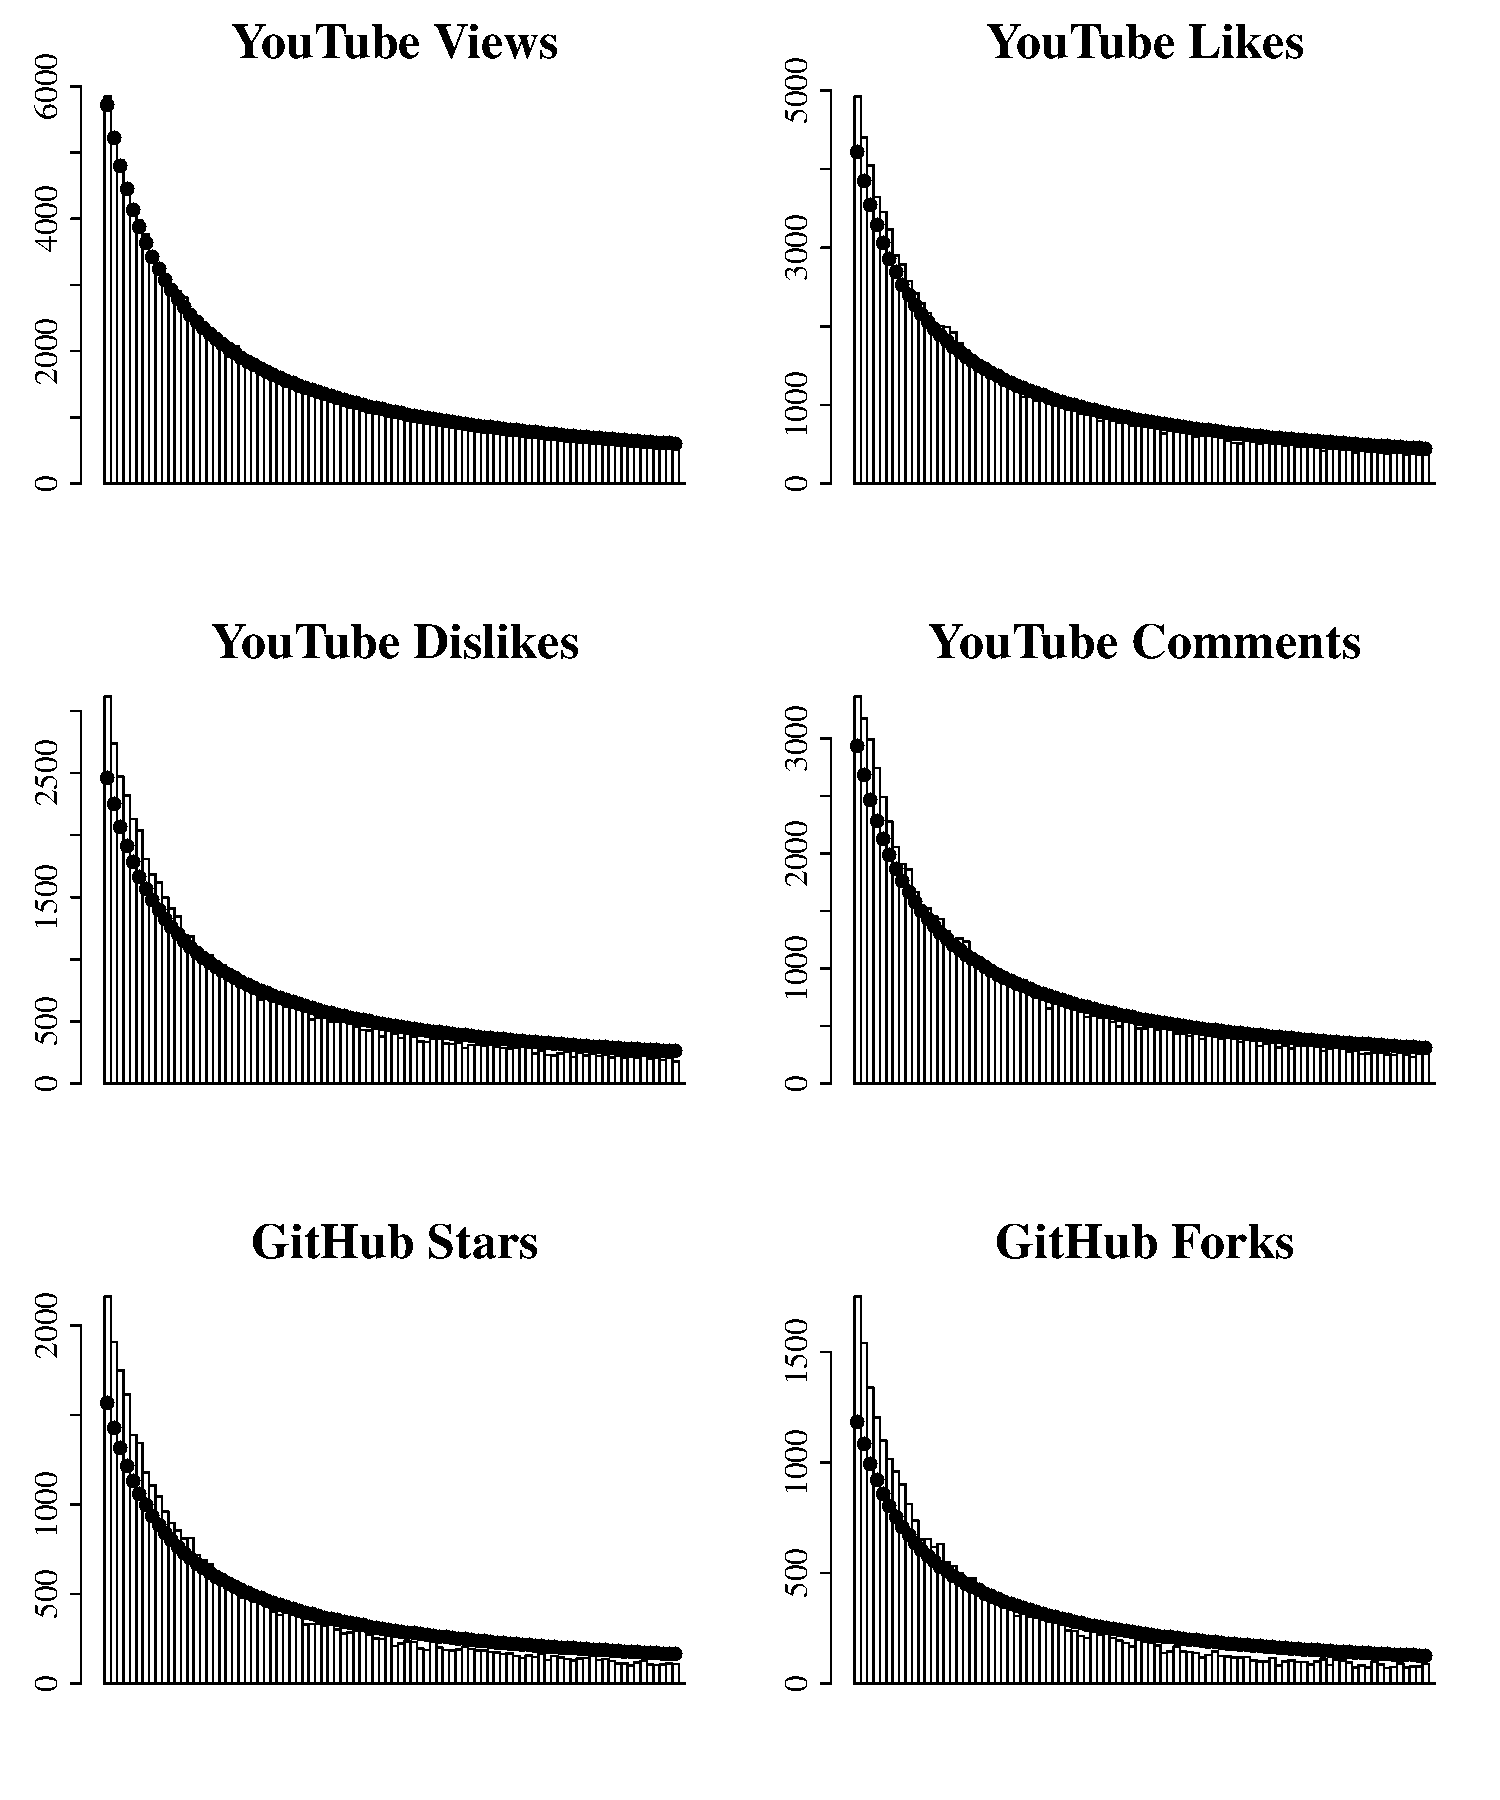
\includegraphics[width=\maxwidth]{figure/github-data-digit-distributions-1} \caption[From top left]{From top left: Leading two-digit histograms for YouTube Views, Likes, Dislikes, Comments, and GitHub Stars and Forks. Each histogram bar on the horizontal axis represents one of the 90 possible leading two digit combinations (10-99).}\label{fig:github-data-digit-distributions}
\end{figure}


\end{knitrout}

% Interestingly, we see that the level of conformity correlates with the range of the metric in question. That is, the YouTube view counts range up to the large value of $signif(max(viewsCount),2)$ and are seen to be a close to perfect fit to Benford's prediction. YouTube likes, dislikes and comment counts, however, span a narrower range. Their maximum values are $signif(max(likesCount),2)$, $signif(max(dislikesCount),3)$ and $signif(max(commentsCount),3)$ respectively. GitHub stars and forks have even narrower ranges (up to $signif(max(starsCount),4)$, $signif(max(forksCount),4)$ and $max(issuesCount)$ respectively). This result empirically helps to support the conjecture that BL is most pronounced for data spanning many orders of magnitude.

\section{Bot-Detection using Benford's Law}
\label{sec:bot-detection-using-benfords-law}

In this section we consider the application of Benford's Law in the detection of anomalous behavior in online services in the form of \textbf{bots} (where automated computer programs, rather than humans, interact with a system). As a case study we present and share data collected from Wikipedia's real-time Recent Changes (RC) stream\footnote{mediawiki.org/wiki/API:Recent\_changes\_stream}. 

Between July 6 and July 11 2016 we collected $n>2$ million page-edit events classified by Wikipedia as \textit{non-bot} edits. We recorded the vector $\vec{\Delta}=\left(\delta_1, \delta_2, \ldots, \delta_n\right)$, where each $\delta_i$ represents the magnitude in bytes of the corresponding change. Changes ranged from a few bytes to over two megabytes. 

% Figure \ref{fig:wikipedia-data-log-histogram} shows the histogram of the \textit{logarithms} of the values in $\vec{\Delta}$.
% 
% wikipedia-data-log-histogram, fig.width=10, fig.height=5, fig.pos='h!', fig.cap='Histogram showing the distribution of the logarithms of the Wikipedia page-edit deltas',echo=F, warning=F
% wikiData <- read.csv("data/wiki-all-length-2016-07-06.csv",header=FALSE)
% # The columns in wikiData represent the server name, bot?, patrolled?, type (edit/new), minor?, old length, new length, delta, comment
% wikiNonBotEdits <- wikiData[wikiData$V2 == 0 & wikiData$V4 == "edit",]
% # Get the vector of deltas
% nonBotEditSizes <- as.numeric(wikiNonBotEdits$V8)
% # Consider the negative deltas only for this experiment (i.e. the destructive changes). Nigrini suggests always analyzing the positive and negative numbers separately. Here we'll analyze negative numbers. We take all those lte -10, so that we can do a two-digit analysis
% nonBotEditSizes <- abs(nonBotEditSizes[nonBotEditSizes<=-10])
% # Calculate the base-10 logarithm of the delta magnitudes
% logVector <- log(nonBotEditSizes,base=10)
% # Plot the histogram of the log vector
% hist(logVector, breaks=seq(0.9,7,0.17),xlab="",main="Logarithms of Page-Edit Deltas",cex.main=2,cex.lab=1.3,cex.axis=1.3)
% @ 

% We see that the distribution of logarithms has the long tail expected from this kind of data (large change deltas are less common). 

\begin{knitrout}
\definecolor{shadecolor}{rgb}{0.969, 0.969, 0.969}\color{fgcolor}\begin{figure}[h!]
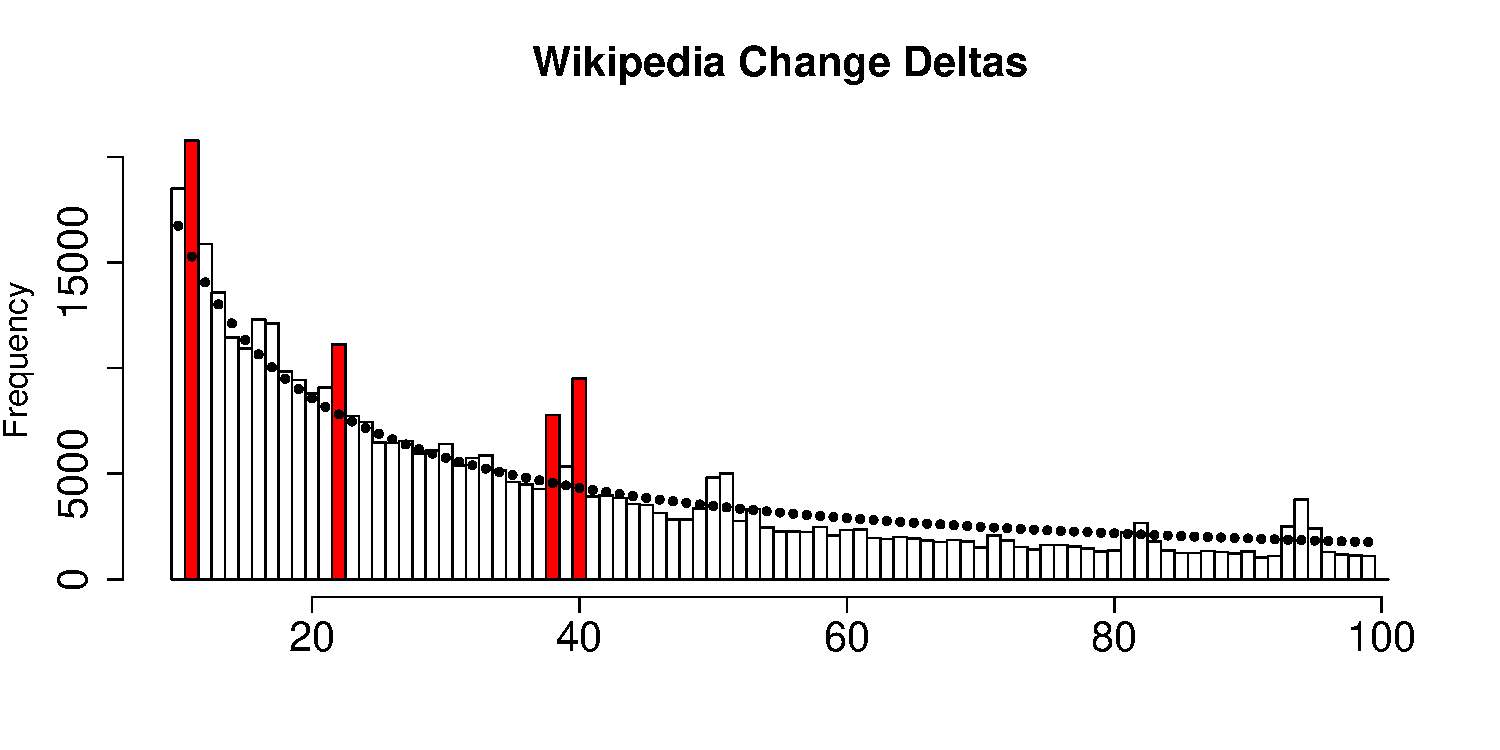
\includegraphics[width=\maxwidth]{figure/wikipedia-data-digits-histogram-1} \caption[Leading two-digit histogram for Wikipedia page-edit deltas]{Leading two-digit histogram for Wikipedia page-edit deltas. Red bars are abberations from BL.}\label{fig:wikipedia-data-digits-histogram}
\end{figure}


\end{knitrout}

Consider in Figure \ref{fig:wikipedia-data-digits-histogram} the distribution of the \textit{leading two digits} of this data. From the basic form of the leading-digits distribution it is evident that the data in question fits the general shape predicted by Benford's Law (again shown by bullets $\bullet$). However, we see some clear aberrations. For example, noticeable spikes exist for the digit pairs $11, 22, 38$ and $40$. This data is therefore a candidate for ``red flagging'' and investigation.

Filtering the data to include only the editor comments for the changes with a delta beginning with the digits $40$, for example, we quickly notice a significant amount of automation happening, despite the edits being flagged by Wikipedia as \textit{non-bot}. Table \ref{tab:wikiBotCommentExamples} contains a sample of the offending comments. We see edits being made by ``Addbots'' as well as tools like HotCat and Gadget-Merge (automated tools for mass-editing Wikipedia content). The byte counts often \textit{begin} with the digits $40$ (despite their full values spanning several orders of magnitude), which manifests as the spike in Figure \ref{fig:wikipedia-data-digits-histogram}. At the very least, Benford's Law has thus uncovered what appears to be a data-integrity issue in the Wikipedia: many automated transactions are not being suitably labeled.

\begin{table}[h!]
  \centering
  \begin{tabular}{|l|l|}
    \hline    
    \textbf{Change comment} & \textbf{Bytes} \\
    \hline
    \footnotesize{\texttt{[[SpiderMum]] [[User:Addbot|Addbot]]}} & \textbf{40} \\
    \footnotesize{\texttt{Removed using [[Gadget-HotCat|HotCat]]}} & \textbf{40} \\
    \footnotesize{\texttt{Wbremoveclaims-remove [[P1012,Q902513]]}} & \textbf{40}7 \\
    \footnotesize{\texttt{[[MediaWiki:Gadget-Merge]] 0||Q75421}} & \textbf{40}62 \\    
    \footnotesize{\texttt{[[OneClickArchiver]]}} & \textbf{40}971 \\    
    \hline
  \end{tabular}
  \caption{Examples of automated Wikipedia edits}
  \label{tab:wikiBotCommentExamples}
\end{table}


\section{Testing Conformity to Benford's Law}
\label{sec:test-conf-benf}



We require a mechanism to objectively assess a given numerical sample's conformity to BL. The ``state-of-the-art'' for such tests was recently surveyed by Nigrini \cite{nigrini2012}. Broadly speaking, one can partition BL tests into three categories: \textit{single-digit} tests, \textit{all-digits-at-once} tests and tests exploiting the \textit{logarithmic basis} of BL. To evaluate these tests, we consider two geometric progressions (i.e. $a^1,a^2,\ldots,a^n$) with common ratios $a=1.2$ and $1.8$. From Section \ref{sec:preliminaries} we know that each sequence obeys BL exactly in the limit $n \rightarrow \infty$.

Table \ref{tab:bl-conformity-tests} displays the conclusions (``Benford'' or ``Non-Benford'') that each test detailed in \cite{nigrini2012} makes for our two sequences based on a significance level of 0.05 and sequence length $n=100$.

\begin{table}[h]
  \tiny
  \centering
  \begin{tabular}[h]{|l|l|l|l|p{2.5cm}|}
    \hline
    Test & Type & Seq. 1 is & Seq. 2 is & Remarks \\
    \hline
    Z-Stat. & Single & \textbf{Benf.} & Non-Benf. & 8 digits deviate significantly for Seq. 2  \\    
    Chi-Sq. & All & \textbf{Benf.} & Non-Benf. & Seq. 2 $\chi^2=22.8$ ($9-1=8$ d.o.f.)\\
    Euc. Dist. & All & \textbf{Benf.} & Non-Benf. & \\
    Hot. $T^2$ & All & \textbf{Benf.} & Non-Benf. & \\
    JP Sq. & All & \textbf{Benf.} & Non-Benf. & \\
    MAD & All & \textbf{Benf.} & Non-Benf. & Critical values from \cite{nigrini2012} \\
    Mant. Arc & Log & \textbf{Benf.} & \textbf{Benf.} &  \\
    K-S Mant. & Log & \textbf{Benf.} & \textbf{Benf.} & \textit{(Our proposed technique)}  \\
    \hline
  \end{tabular}
  \caption{Comparison of BL-conformity tests on two geometric progressions}
  \label{tab:bl-conformity-tests}
\end{table}

The tests based on the \textit{discrete digit distribution} (``Single'' digit, or ``All'' at once) fail to label the second sequence as Benford. These techniques are the Z-Statistic, Chi-Square, Euclidean Distance, Hotelling T-square, Joenssen's JP-square and Mean Absolute Deviation (MAD) tests. The conflicting conclusions are troublesome because both sequences are non-random and follow ideal exponential growth. The reason for the conflict is that we selected the second common ratio to maximize the \textit{information-loss during the discretization}. For example, we have a large information-loss when discretizing the sequence value 9.8595 to the ``first digit 9'' histogram bin. For moderate sample sizes, these discretization errors are enough to change the leading-digit distribution to the extent that these digits-based tests believe that the sequence is non-Benford.

To overcome this weakness, we argue that a BL conformity test should avoid such a discretization. In this light, we can design tests around the \textit{logarithmic basis} of BL, which states that the mantissae\footnote{The mantissa of a number is the fractional part of its logarithm.} of a Benford set are uniformly distributed over $[0,1)$.

Nigrini \cite{nigrini2012} also discusses BL tests that exploit this logarithmic basis. The first involves testing for two conditions: if the mantissae have a uniform distribution, then their mean and variance must be $\frac{1}{2}$ and $\frac{1}{12}$ respectively. Nigrini correctly comments that these conditions are insufficient (numerous non-uniform distributions satisfy them) and dismisses this approach. 

% A second mechanism is based on a regression approach  the insight that the ordered (ranked) mantissae should form a straight line from $\frac{-1}{n}$ to $\frac{n-1}{n}$ with a slope of $\frac{1}{n}$. Nigrini hence suggests performing a linear regression on the mantissae and testing the intercept and slope. However, a regression-based test ``should only be used after more research'' \cite{nigrini2012}. 

Another logarithmic-basis test discussed by Nigrini is the recent Mantissa-Arc (Mant. Arc) test \cite{alexander2009remarks}. It involves projecting the mantissae around the circumference of the unit circle and testing if the center-of-gravity differs significantly from zero. We see in Table \ref{tab:bl-conformity-tests} that the Mantissa-Arc test is able to correctly diagnose both sequences as Benford. At first glance, this test appears promising, however we soon realize that the center-of-gravity condition is insufficient. Consider, for example, the arbitrary-length sample $10^{1/4},10^{3/4},10^{1/4},10^{3/4},\ldots,10^{1/4},10^{3/4}$ having only two unique values. These two values are mapped to opposite sides of the unit circle, giving a zero center-of-gravity and incorrectly signaling \textit{perfect} Benford conformity. We therefore suggest to avoid this test.

Why not apply a test which directly compares the empirical cumulative distribution of the mantissae with the cumulative distribution function of the uniform? To the best of our knowledge, this approach has not been suggested. Specifically, we propose applying the formal Kolmogorov-Smirnov (K-S) one-sample test \cite{kolmogorov1933} on the mantissae to test whether or not they were sampled from the uniform. Here the null hypothesis is that the mantissae were drawn from the uniform. Adopting the common significance threshold $\alpha=0.05$, we interpret a $p<\alpha$ as an indicator for non-Benfordness. Consider for example our Twitter status-count mantissae:

%% Various classical and specialized tests can be used to this end. We refer to Nigrini's recent work \cite{nigrini2012} for a detailed discussion on such tests. One recommendation from this reference is the \textit{Mean Absolute Deviation} (MAD) test. This test yields a MAD statistic, which, as hinted in the name, is the average of the magnitudes of the differences between the observed digit proportions and those predicted by BL. In Figure \ref{fig:twitter-count-distributions}, for example, the statistic is simply calculated by summing up the distances between the each bullet/bar pair, and dividing by nine (the number of possible first digits). Smaller values of the MAD correspond to higher Benfordness. Although simple to compute, the MAD is not able to provide us with objective critical values for statistical significance (a key requirement for an event-detection framework).

\noindent
\begin{knitrout}
\definecolor{shadecolor}{rgb}{0.969, 0.969, 0.969}\color{fgcolor}
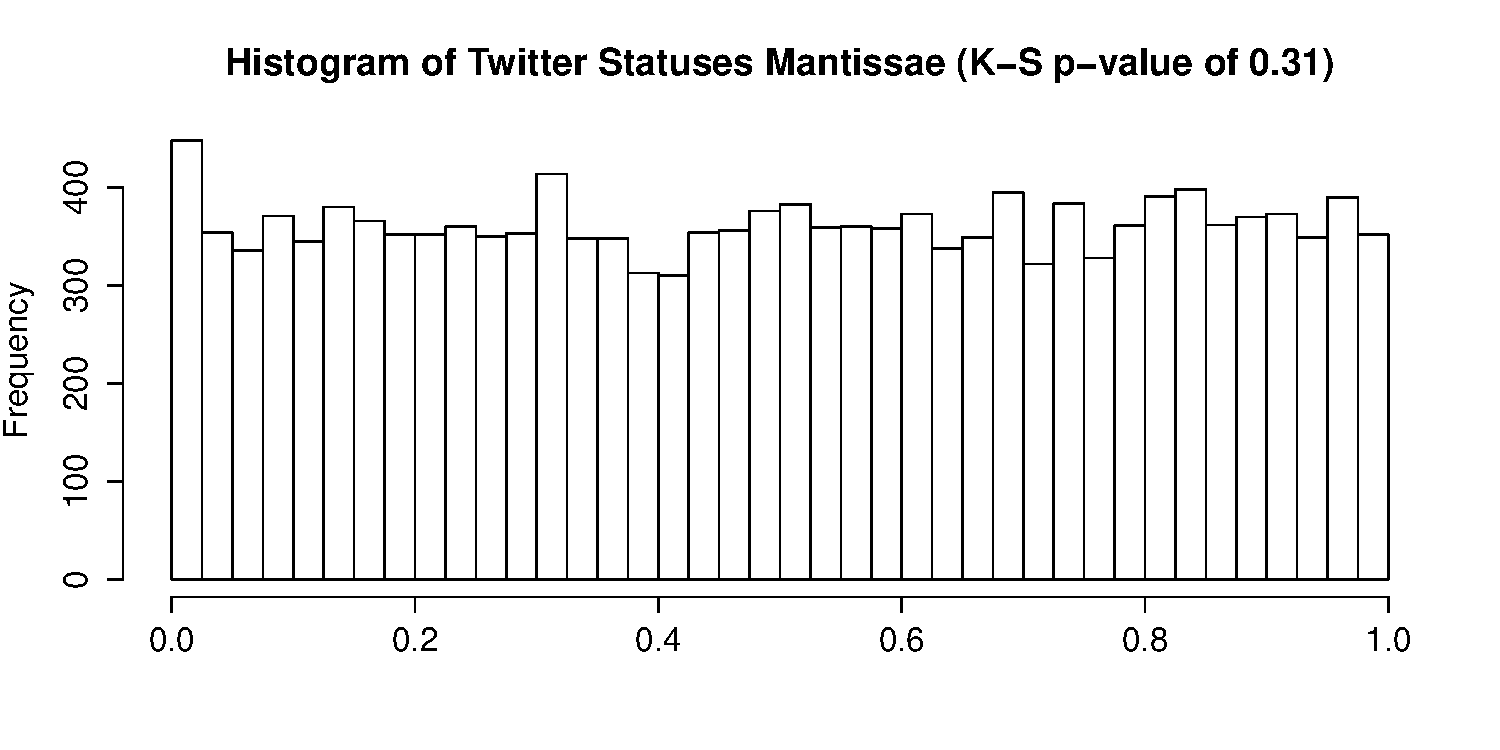
\includegraphics[width=\maxwidth]{figure/conformity-test-twitter-example-1} 

\end{knitrout}

The $p$-value corresponding to the application of the K-S test on this sample is 0.31. We hence accept our null hypothesis that the sample was taken from a uniform distribution, and hence that the sample conforms to BL. This same approach correctly diagnoses both our test sequences as Benford (final row in Table \ref{tab:bl-conformity-tests}). We note that the application of the K-S test on a sample involves no obscure parameters -- we only need a significance threshold $\alpha$ in order to reach a conclusion for a sample.

\section{From a Time Series to a Benfordness Signal}
\label{sec:extr-benf-sign}

Equipped with a tool to measure the Benfordness of a univariate sample, we now turn to the real-time detection of ``non-Benford'' events. That is, we wish to be alerted when a significant deviation from the ``natural'' state of a running system occurs. 

To achieve this, we track key metrics over time (e.g. follower counts of tweeting users) and apply the K-S Test on a sliding time window. The time window contains a fixed number $w$ of the newest numeric values. For the sample of size $w$ corresponding to each window, we compute the mantissae and apply the K-S test as discussed in Section \ref{sec:test-conf-benf}. The resulting $p$-value is the quantity that we then follow over time. We interpret a drop of the $p$-value below a significance threshold $\alpha$ as an indicator for the beginning of ``non-Benford'' behavior in the system (something unnatural that should be investigated).

\textbf{Window Size $w$ and Threshold $\alpha$:} The value for $w$ is user-specified. The K-S test we use for BL-conformity has an asymptotic power of 1. For $w \rightarrow \infty$ this implies that there is zero probability of rejecting a true null hypothesis. In practice, however, a large value of $w$ means that we miss out on potentially important dynamics of the system under investigation. At the other extreme, if $w$ is too small, we lack statistical power and thus have a higher false negative rate. As always, $w$ should be chosen considering this trade-off and the application. For our upcoming Twitter case studies (Sections \ref{sec:case-study:-twitter} and \ref{sec:case-study:-outag}), we will see that a common window size ($w=2000$) was sufficient.

The value for $\alpha$ can likewise be user-specified, however we will see in real-world case studies (Figure \ref{fig:case-study-pokemon}) and synthetic experiments (Figure \ref{fig:synthetic-experiments}) that similar results are obtained for the commonly-chosen threshold levels ($\alpha=0.01,0.05$). We use $\alpha=0.05$ in all our work.

\subsection{Performance}
\label{sec:performance}

Assuming a fixed significance threshold $\alpha$ and window size $w$, the K-S critical value can be computed in advance using existing tables for the K-S statistic distribution (for $\alpha=0.05$ it is $\frac{1.358}{\sqrt{w}}$, for example). Our optimized implementation of \algoname{} hence works directly with the K-S statistic, avoiding the need to compute $p$-values.

To calculate the K-S statistic for the current window we would normally need to sort its contents. Using a comparison-based sorting procedure like Heapsort implies a $\mathcal{O}(w \cdot \log w)$ run-time in the worst case for this step. In practice, this sorting only needs to be performed once for the first window. Afterwards, we use standard indexing structures to update our sorted window in $\mathcal{O}(1)$ operations. For each new stream value the calculation of the K-S statistic is hence reduced to $\mathcal{O}(w)$, which is the time to determine the maximum difference between the window's ECDF and the reference uniform distribution.


\section{Case Study: Hashtag Hijacking}
\label{sec:case-study:-twitter}

In the context of social media, Hashtag Hijacking occurs when a hashtag is (ab)used for purposes other than intended. We now demonstrate \algoname{}'s ability to detect this phenomenon in real-time.

\begin{knitrout}
\definecolor{shadecolor}{rgb}{0.969, 0.969, 0.969}\color{fgcolor}\begin{figure}[t!]
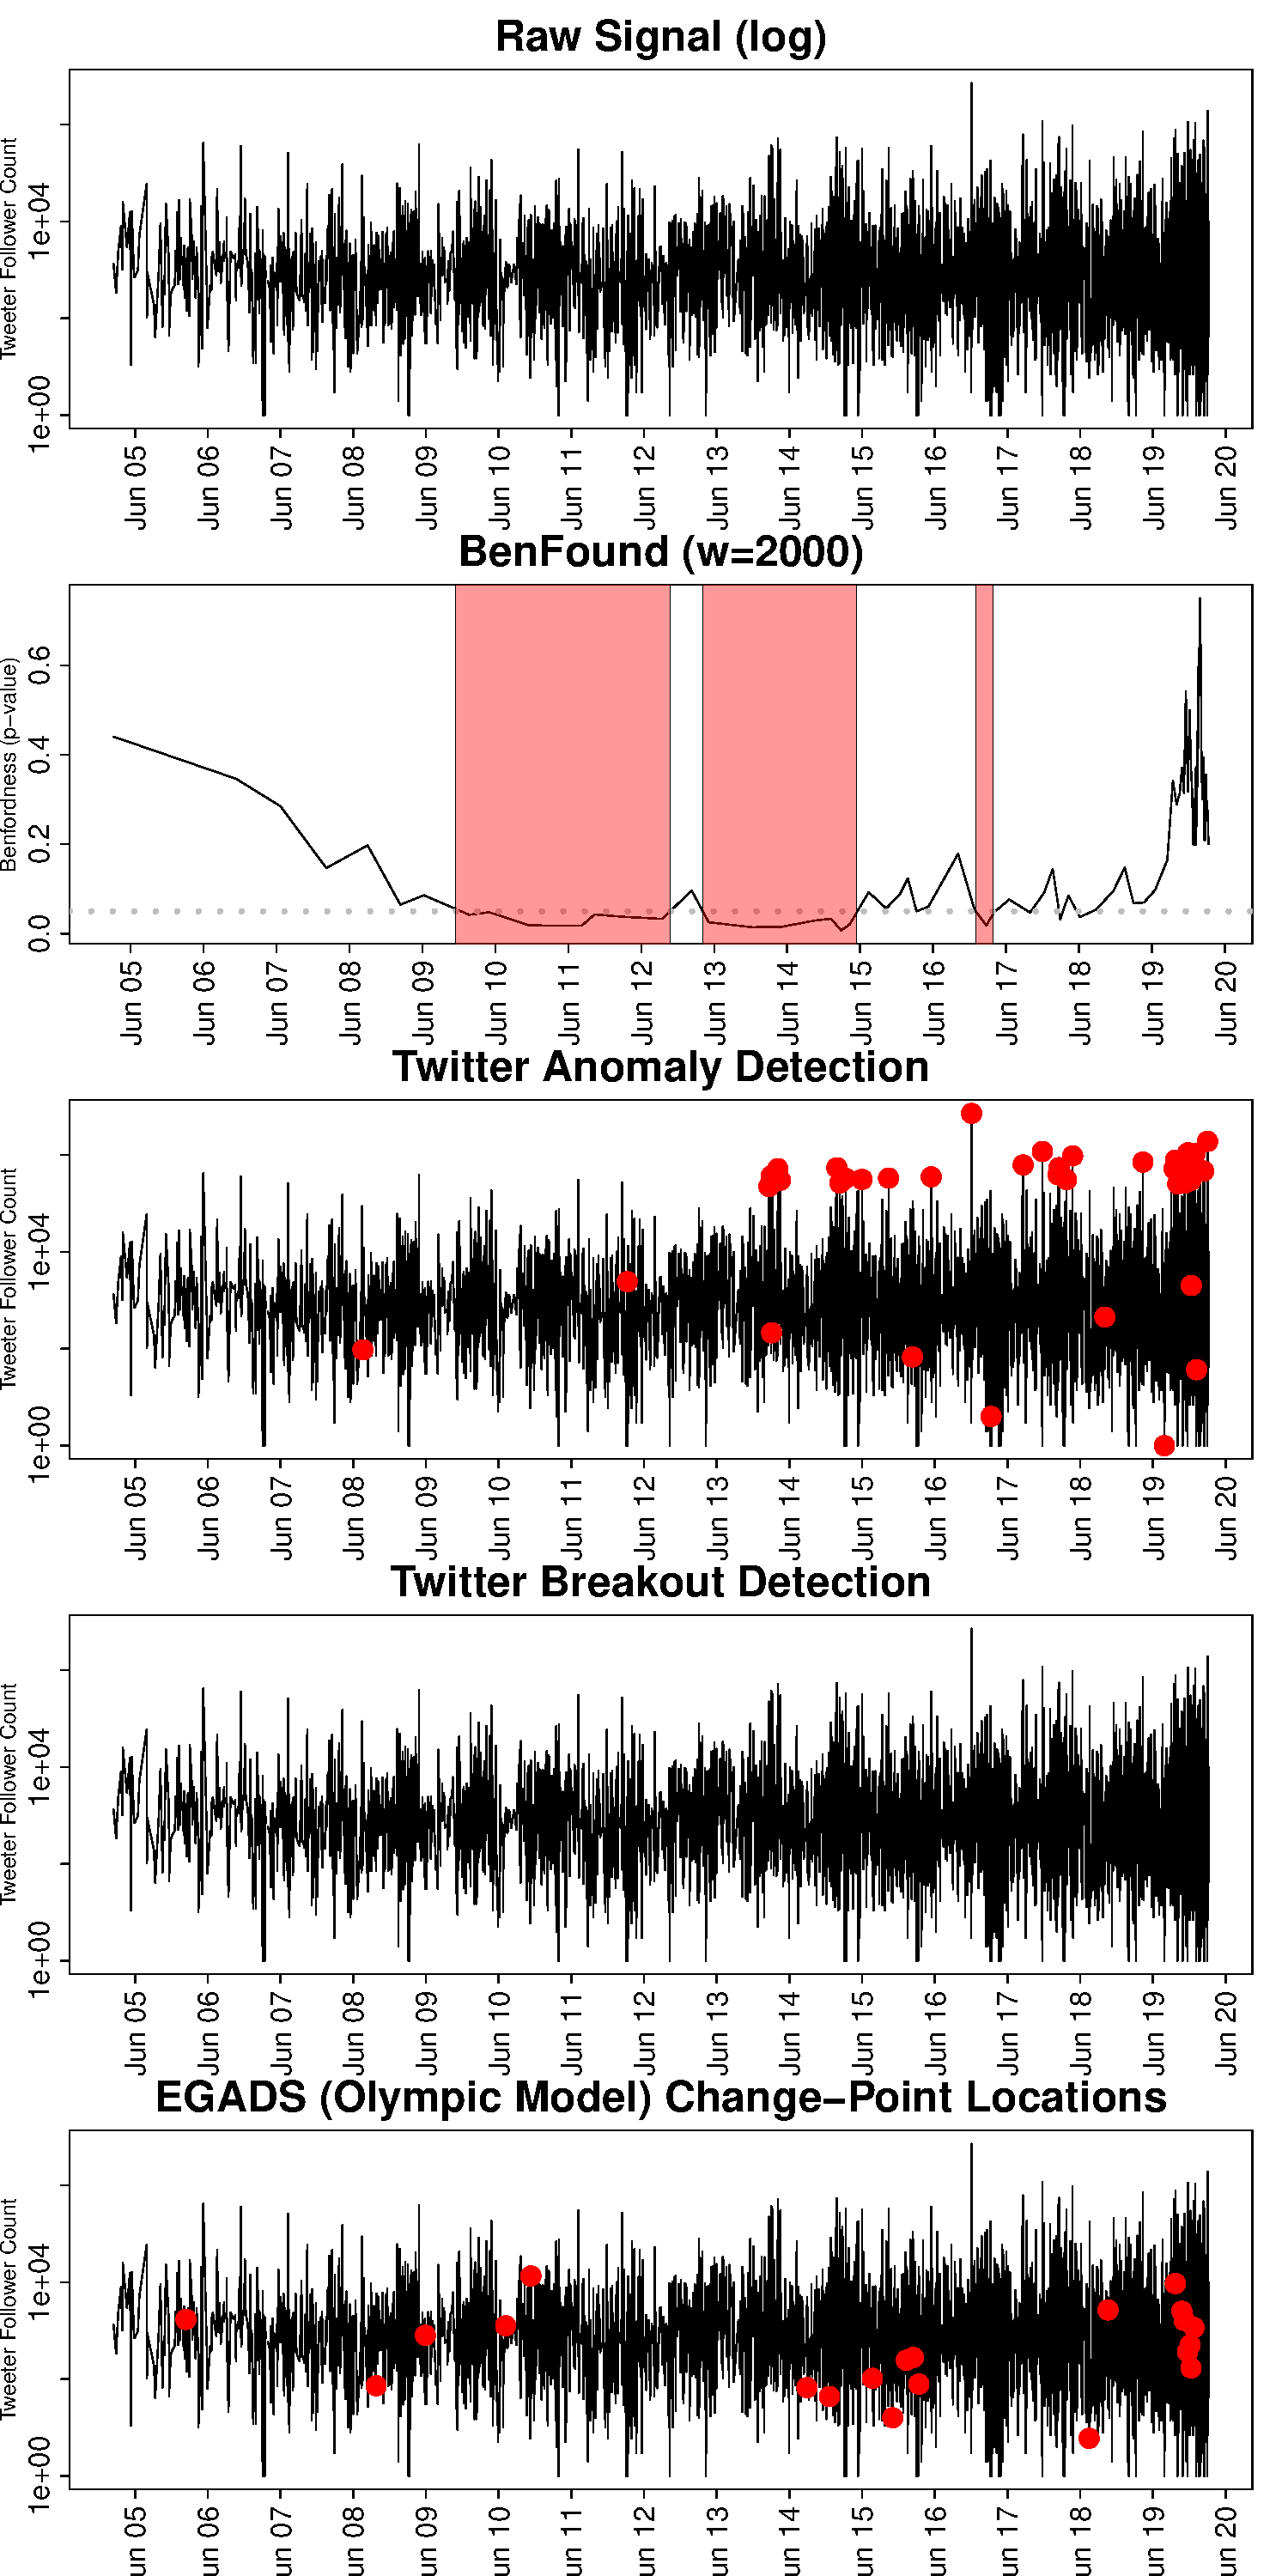
\includegraphics[width=\maxwidth]{figure/case-study-hashtag-hijacking-twitter-1} \caption[Raw follower counts (top) for users tweeting the hashtag FathersDay]{Raw follower counts (top) for users tweeting the hashtag FathersDay. The remaining plots show events, anomalies and changepoints detected by BenFound and other approaches.}\label{fig:case-study-hashtag-hijacking-twitter}
\end{figure}


\end{knitrout}

Consider the hashtag \textbf{\#FathersDay}. The intended purpose of this hashtag is to allow Twitter users to celebrate their father. Father's Day occurred in most countries on 19 June 2016. During the time leading up to Father's Day, we listened for and logged all tweets referencing this hashtag. The raw follower counts of the corresponding tweeters are traced in Figure \ref{fig:case-study-hashtag-hijacking-twitter}. The same Figure shows events, anomalies and change-points found by \algoname{} and three state-of-the-art approaches (\cite{laptev2015egads,james2014twitter,vallis2014novel}, discussed further in Section \ref{sec:synth-exper} and \ref{sec:related-work}). These three approaches consider the \textit{absolute values} of the streamed values (tweeter follower counts).

The \algoname{} signal shows that the behavior begins Benford, turning non-Benford before Father's Day, and finally regressing to Benford \textit{on} Father's Day. Looking at the data, we quickly see the behavior that the Benfordness signal describes. In the lead-up to Father's Day, a large number of spammers and advertising accounts hijacked the hashtag. The follower-counts of these accounts have a non-Benford (unnatural) digit distribution. This behavior is reflected in the low $p$-value of the Benfordness signal. It first drops below our threshold on 10 June 2016\footnote{We note that times were not measured in an American timezone (rather UTC), hence the reason for the slight shift in the data.}, the beginning of the weekend before Father's Day and a logical time for those spammers and advertisers unscrupulously trying to generate profit from the event to begin pushing their content. Example tweets from this time are in Table \ref{tab:sampleTweetsFathersDayLeadUp}.

On Father's Day itself, spammers and advertisers presumably recognized that time had run out to generate profit from this hashtag. The tweet behavior shifted to the more organic kind of content expected for this hashtag. In Table \ref{tab:sampleTweetsFathersDayLeadUp} we find examples of the tweets from 19 June 2016 (users celebrating the efforts of fathers).

The other techniques struggle to extract meaningful information from the raw signal. Two of the techniques find an indigestible number of changepoints/anomalies; the third (Breakout Detection) finds none at all.

\begin{table}[h!]
  \footnotesize
  \centering
  \begin{tabular}{|p{8cm}|}
    \hline
    \textbf{\underline{Father's Day lead-up:}} \\
    \textit{``Oh Yea! I just entered to \#Win LED GlowBowl''}; \textit{``Check out Libbey Ceramic Tiki Mug Blue 7 x 3 16 Ounces''}; \textit{``Enter the \#giveaway to \#win''}; \textit{``I just entered to \#win a \$50 giftcard to @cuffdaddy \#giveaway''}; \\
    \textbf{\underline{Father's Day itself:}} \\
    \textit{``I love you Dad, Happy Father's Day''}; \textit{``The best thing a man can do for his children is to love their mother''}; \textit{``To all of the champion fathers... Happy \#FathersDay!''}; \textit{``Hope you had a great \#FathersDay, lads!''}  \\
    \hline
  \end{tabular}
  \caption{Tweets \textit{leading up to} and \textit{on} Father's Day}
  \label{tab:sampleTweetsFathersDayLeadUp}
\end{table}


\section{Case Study: Outage Detection}
\label{sec:case-study:-outag}

Shortly before the time of data collection, the popular \textbf{\#PokemonGO} game had been released. We tracked the tweets to this hashtag over a number of days. The Benfordness signal is shown in Figure \ref{fig:case-study-pokemon}.

The signal shows a sharp drop on July 15 and 16, hinting that the ``natural'' behavior of tweets for this hashtag had changed. An analysis of the data reveals that the the Pokemon GO application suffered severe outages during this time period. The tweets during this time period were largely revolving around these problems (see Table \ref{tab:sampleTweetsPokemon}) and had a non-Benford digit distribution. The official \textbf{@PokemonGoApp} account confirmed the problems on July 16 (Figure \ref{fig:twitter-pokemongoapp-tweets}). As a comparison, the state-of-the-art Twitter Anomaly Detection result is shown in Figure \ref{fig:case-study-pokemon}, and events/topics detected using two state-of-the-art Twitter text-mining approaches are shown in Table \ref{tab:top10NlpPokemon}.

\begin{knitrout}
\definecolor{shadecolor}{rgb}{0.969, 0.969, 0.969}\color{fgcolor}\begin{figure}[t]
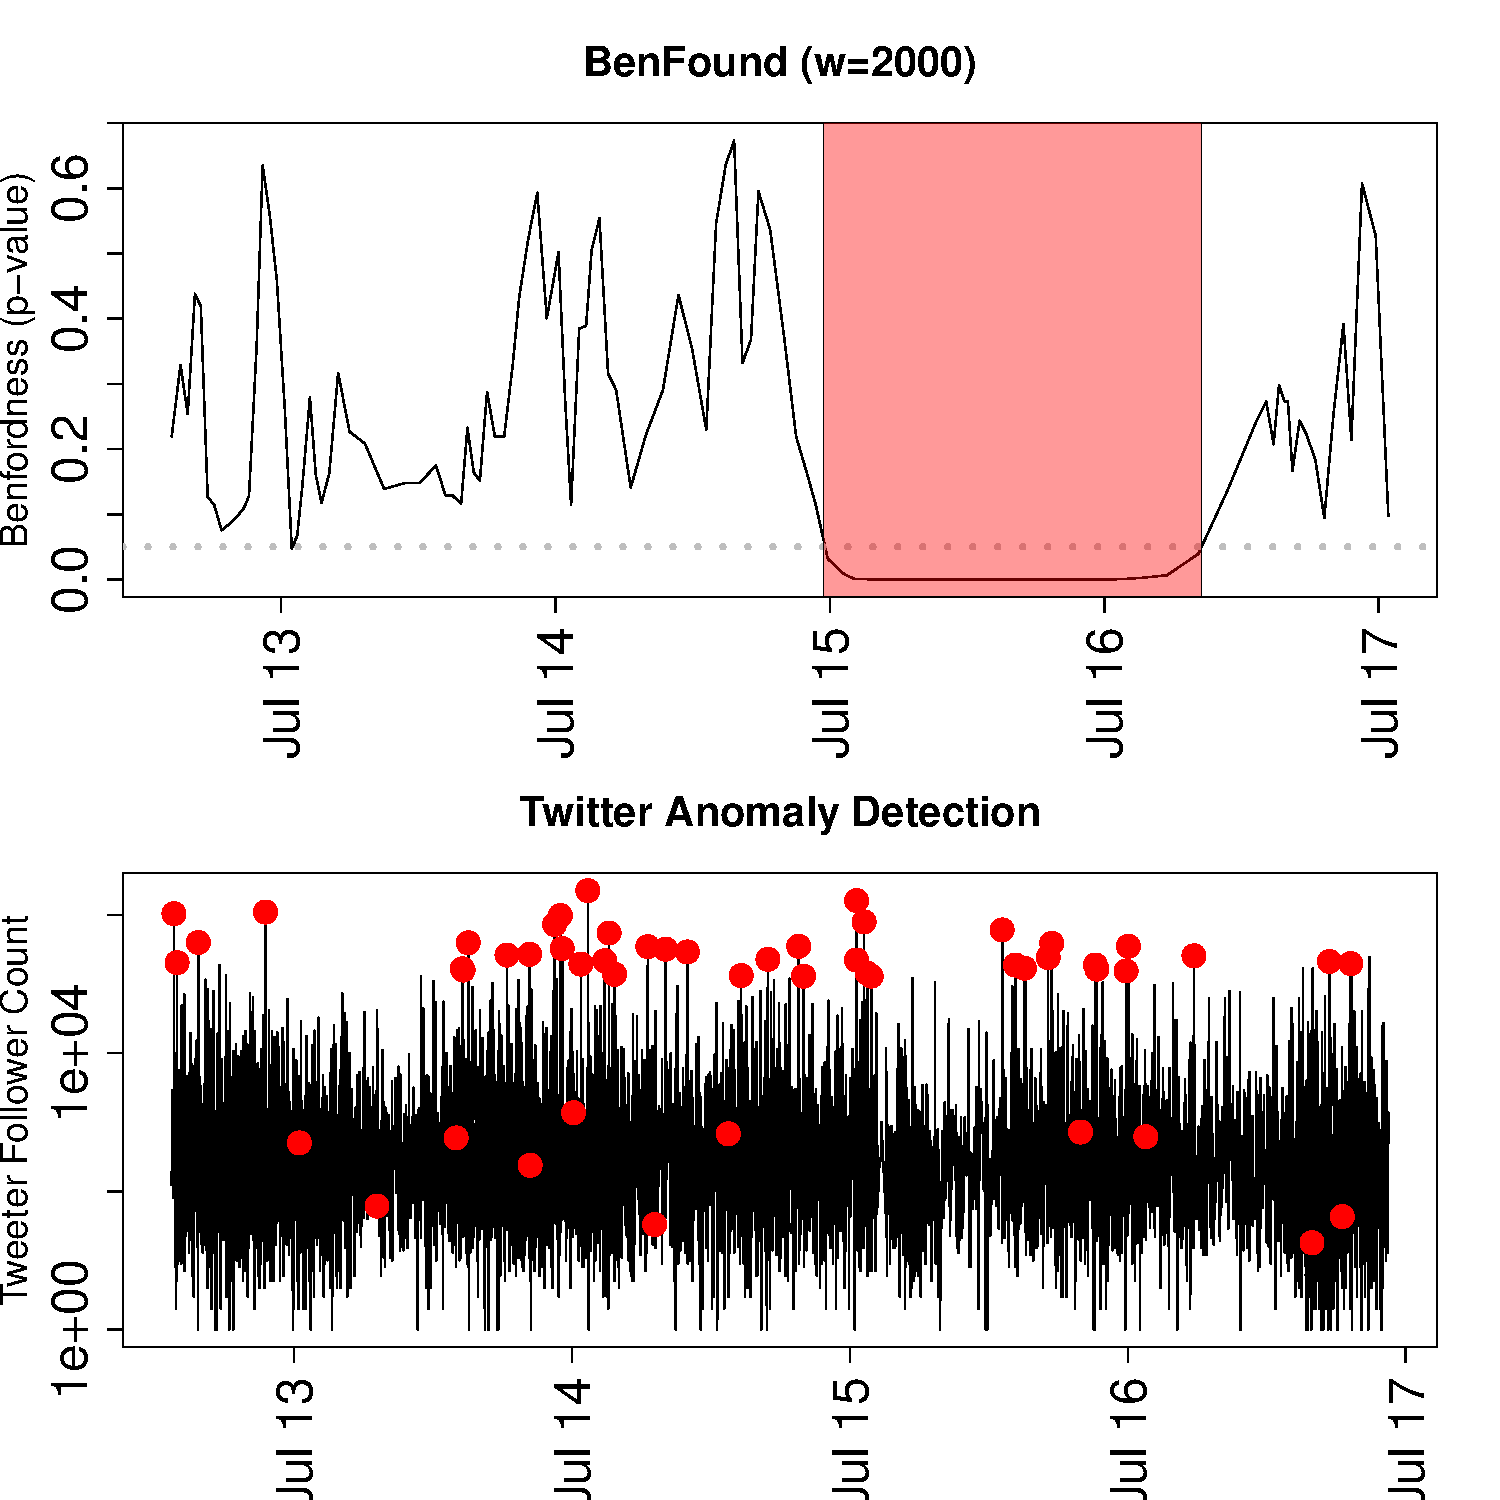
\includegraphics[width=\maxwidth]{figure/case-study-pokemon-1} \caption[Tracking the Benfordness of follower-counts associated with users tweeting against the \#PokemonGO hashtag]{Tracking the Benfordness of follower-counts associated with users tweeting against the \#PokemonGO hashtag.}\label{fig:case-study-pokemon}
\end{figure}


\end{knitrout}

\begin{table}[h!]
  \footnotesize
  \centering
  \begin{tabular}{|p{8cm}|}
    \hline
    \textit{SERVER UPDATE: According to @Independent, \#PokemonGO servers have been taken down in a DDOS attack.} \\
    \textit{The \#PokemonGO servers are down due to a DDOS attack. No word on when they will be back. Stay with us for the latest.} \\
    \textit{Niantic trying to fix the \#PokemonGO servers is as successful as Team Rocket trying to kidnap Pikachu.} \\
    \textit{\#PokemonGO is down. What do I do now with my time?} \\
    \hline
  \end{tabular}
  \caption{Sample of Tweets with the hashtag \#PokemonGO on July 15 and 16, 2016}
  \label{tab:sampleTweetsPokemon}
\end{table}

\begin{table}[h!]
  \footnotesize
  \centering
  \begin{tabular}{|p{8cm}|}
    \hline
    \textbf{Top 10 (Twitter NLP \cite{ritter2012open})}: has in, strict parents, bringing out, \textbf{are down}, came over, get off, \textbf{go down}, looking for, \textbf{been down}, get out \\
    \textbf{Top 10 (Twitter Topic Detection (Streaming NMF) \cite{hayashi2015real})}: [argentina, coins, nintendome], [team, argentina, spark], [pokemongonews, argentina, community], [pokecoins, try, need], [argentina, giveaway, must], [try, \textbf{servers}, pokecoins], [syrian, hopes, saved], [argentina, coins, lucky], [argentina, need, try], [argentina, \textbf{unstable}, lucky]\\
    \hline
  \end{tabular}
  \caption{Top 10 events/topics found by two state-of-the-art Twitter text-mining techniques \cite{hayashi2015real,  ritter2012open}.}
  \label{tab:top10NlpPokemon}
\end{table}

\begin{figure}[h!]
  \centering
  
\includegraphics[width=0.8\maxwidth]{graphics/TwitterPostsPokemon.png} \caption[Tweets from the verified \@PokemonGoApp account on July 16, 2016.]{Tweets from the verified \@PokemonGoApp account on July 16, 2016.}\label{fig:twitter-pokemongoapp-tweets}
\end{figure}


\section{Experiments on Synthetic Data}
\label{sec:synth-exper}

In this section we use synthetically-generated numerical time-series data to compare our proposed method with state-of-the-art techniques from the field of numerical event- and anomaly-detection. Our generative model is inspired by our observations from online services such as Wikipedia and Twitter. From our introduction we know that normal usage patterns in these services lead to highly-Benford metrics. In contrast, the set of such values coming from ``unnatural'' usage patterns like bots and hashtag-hijacking is often non-Benford. Our goal is to be alerted when such non-Benford changes occur (denoted a \textit{negative} event), as well as when things return to being Benford (denoted a \textit{positive} event). We make all synthetic models, data and experiments that follow available for reuse\footnotemark[\ref{supMatFootnote}].

We make the simplifying assumption that one interaction (e.g. page edit in Wikipedia or tweet in Twitter) occurs per unit of time. The $n$ interactions with the system fall at times $t_1, \ldots, t_n$. To evaluate the detection of both \textit{negative} and \textit{positive} events, we divide time into \textbf{three intervals}. The first interval spans the range $t_1,\ldots,t_{\lfloor\frac{n}{3}\rfloor}$, the second $t_{\lfloor\frac{n}{3}\rfloor + 1},\ldots,t_{\lfloor\frac{2n}{3}\rfloor}$ and the third $t_{\lfloor\frac{2n}{3}\rfloor + 1},\ldots,t_n$. Inside the first and third intervals we generate ``natural'' (Benford) data. For the second interval we generate non-Benford data. In this way we synthesize a negative event at the transition from the first interval to the second, followed by a positive event at the transition from the second interval to the third.

%% With reference to our \textbf{\#FathersDay} example, we recognize that a shift in the \textit{scale} of the followers distribution is no cause for alarm, as long as the digits pattern continues to obey BL. To simulate this, we thus split the first interval into two equally-sized sub-intervals, the only difference being the value range over which the Benford data is generated. For the second interval we generate non-Benford data by sampling from the uniform. The data generation for the third interval is identical to the first. In this way we synthesize a negative event at the transition from the first interval to the second, followed by a positive event at the transition from the second interval to the third.

To generate Benford data for \textbf{intervals one and three}, we begin with a uniformly-distributed sample $\vec{u} \in [0,1]^s$. With reference to Section \ref{sec:test-conf-benf}, this sample $\vec{u}$ represents our mantissae. Next we generate the sample $\vec{m} \in \left\{0,1,\ldots, 10\right\}^s$ of integers (uniformly sampled with replacement). This sample $\vec{m}$ represents our ``magnitude'' information. Our final Benford set of values then satisfies $\log_{10}(\vec{b}) = \log_{10}(\vec{u} + \vec{m})$, thus $\vec{b} = \left(10^{u_1+m_1}, \ldots, 10^{u_s+m_s} \right)$.

To generate \textit{non-Benford} data for \textbf{interval two}, we follow \cite{berger2011benford} and \textit{uniformly} sample in the range $[0,10^{11}]$.

Figure \ref{fig:synthetic-experiments} compares \algoname{} with 10 different approaches/configurations to event and change-point detection. For this data we are not able to compare with techniques specific for social media (e.g. Twitter) because they rely on the text feed and particular features (hashtags, retweets). \algoname{} is the only approach able to identify the correct number of changepoints (two), their locations and the fact that they form a single ``event''. With respect to \textbf{runtime}, \algoname{}'s bandwidth is 8900 streamed values per second when using our R prototype with window size $w=250$. Doubling to $w=500$ reduces the bandwidth to 7850 streamed values per second. As a real-world reference, we note that around 6000 tweets are tweeted on Twitter every second\footnote{internetlivestats.com/twitter-statistics}.

% REPRODUCING THE BANDWIDTH RESULT STATED ABOVE (e.g. 8900 values per second):
% The following code can be used to simulate an online scenario. The first part just generates some synthetic data (length 6000). The second part actually conducts the experiment with increment=1. Note we have to sort once at the beginning before bringing the stream "online"

% totalLength <- 6000; beta1 <- 10; beta2 <- 10; betaNonBenford <- 10;windowSize <- 250; greenRedGreenColors <- rainbow(3,alpha=0.3); greenRedGreenColors <- c(greenRedGreenColors[2],greenRedGreenColors[1], greenRedGreenColors[2]); set.seed(336); vecU <- seq(0,1,length=totalLength/6); vecM11 <- sample(1:beta1,length(vecU),replace=TRUE); vecM12 <- sample(1:beta2,length(vecU),replace=TRUE); vecM21 <- sample(1:beta1,length(vecU),replace=TRUE); vecM22 <- sample(1:beta2,length(vecU),replace=TRUE); vecB11 <- 10^(vecU+vecM11); vecB12 <- 10^(vecU+vecM12); vecB21 <- 10^(vecU+vecM21); vecB22 <- 10^(vecU+vecM22); perfectBenfordSet11 <- sample(vecB11,length(vecB11)); perfectBenfordSet12 <- sample(vecB12,length(vecB12)); perfectBenfordSet21 <- sample(vecB21,length(vecB21)); perfectBenfordSet22 <- sample(vecB22,length(vecB22)); timeSeriesVector <- c(perfectBenfordSet11, perfectBenfordSet12, runif(totalLength/3,0)*10^(sample(2:(betaNonBenford+1),totalLength/3,replace=TRUE)), perfectBenfordSet21,perfectBenfordSet22); 

% windowStarts <- seq(1,length(timeSeriesVector)-windowSize+1,1); currentWindow <- timeSeriesVector[1:windowSize]; currentWindow <- log(currentWindow, 10)-floor(log(currentWindow,10)); currentWindowSorted <- sort(currentWindow); benfordnessSignalIndex <- 1; benfordnessSignal <- numeric(totalLength-windowSize+1); benfordnessSignal[benfordnessSignalIndex] <- calculateKsOneSidedStatisticUniform(currentWindowSorted); uniformEcdfSteps <- (0:(windowSize - 1))/windowSize; inverseWindowSize <- 1/windowSize; timeStart <- proc.time(); for(newValueIndex in (windowSize+1):length(timeSeriesVector)){ benfordnessSignalIndex <- benfordnessSignalIndex+1; newValue <- timeSeriesVector[newValueIndex]; newValue <- log(newValue, 10)-floor(log(newValue,10)); shiftSortedWindowResult <- shiftSortedWindow(currentWindow,currentWindowSorted,newValue); currentWindow <- shiftSortedWindowResult$newWindowUnsorted; currentWindowSorted <- shiftSortedWindowResult$newWindowSorted; differenceToUniform <- punif(currentWindowSorted) - uniformEcdfSteps; ksStatistic <- max(c(differenceToUniform, inverseWindowSize - differenceToUniform));  benfordnessSignal[benfordnessSignalIndex] <- ksStatistic; }; timeEnd <- proc.time(); plot(seq_along(benfordnessSignal),benfordnessSignal,type="l",main="BenFound (statistic,w=250)",xlab="",xaxt="n",ylab="BenFound (p-value)",cex.main=1.5); abline(1.358/sqrt(windowSize),0,col=8,lty=3,lwd=4); print(totalLength/(as.numeric(timeEnd-timeStart)[3])); 



% Note: if isExtendedVersion false, change the figure* to figure below
\begin{knitrout}
\definecolor{shadecolor}{rgb}{0.969, 0.969, 0.969}\color{fgcolor}\begin{figure}[h!]
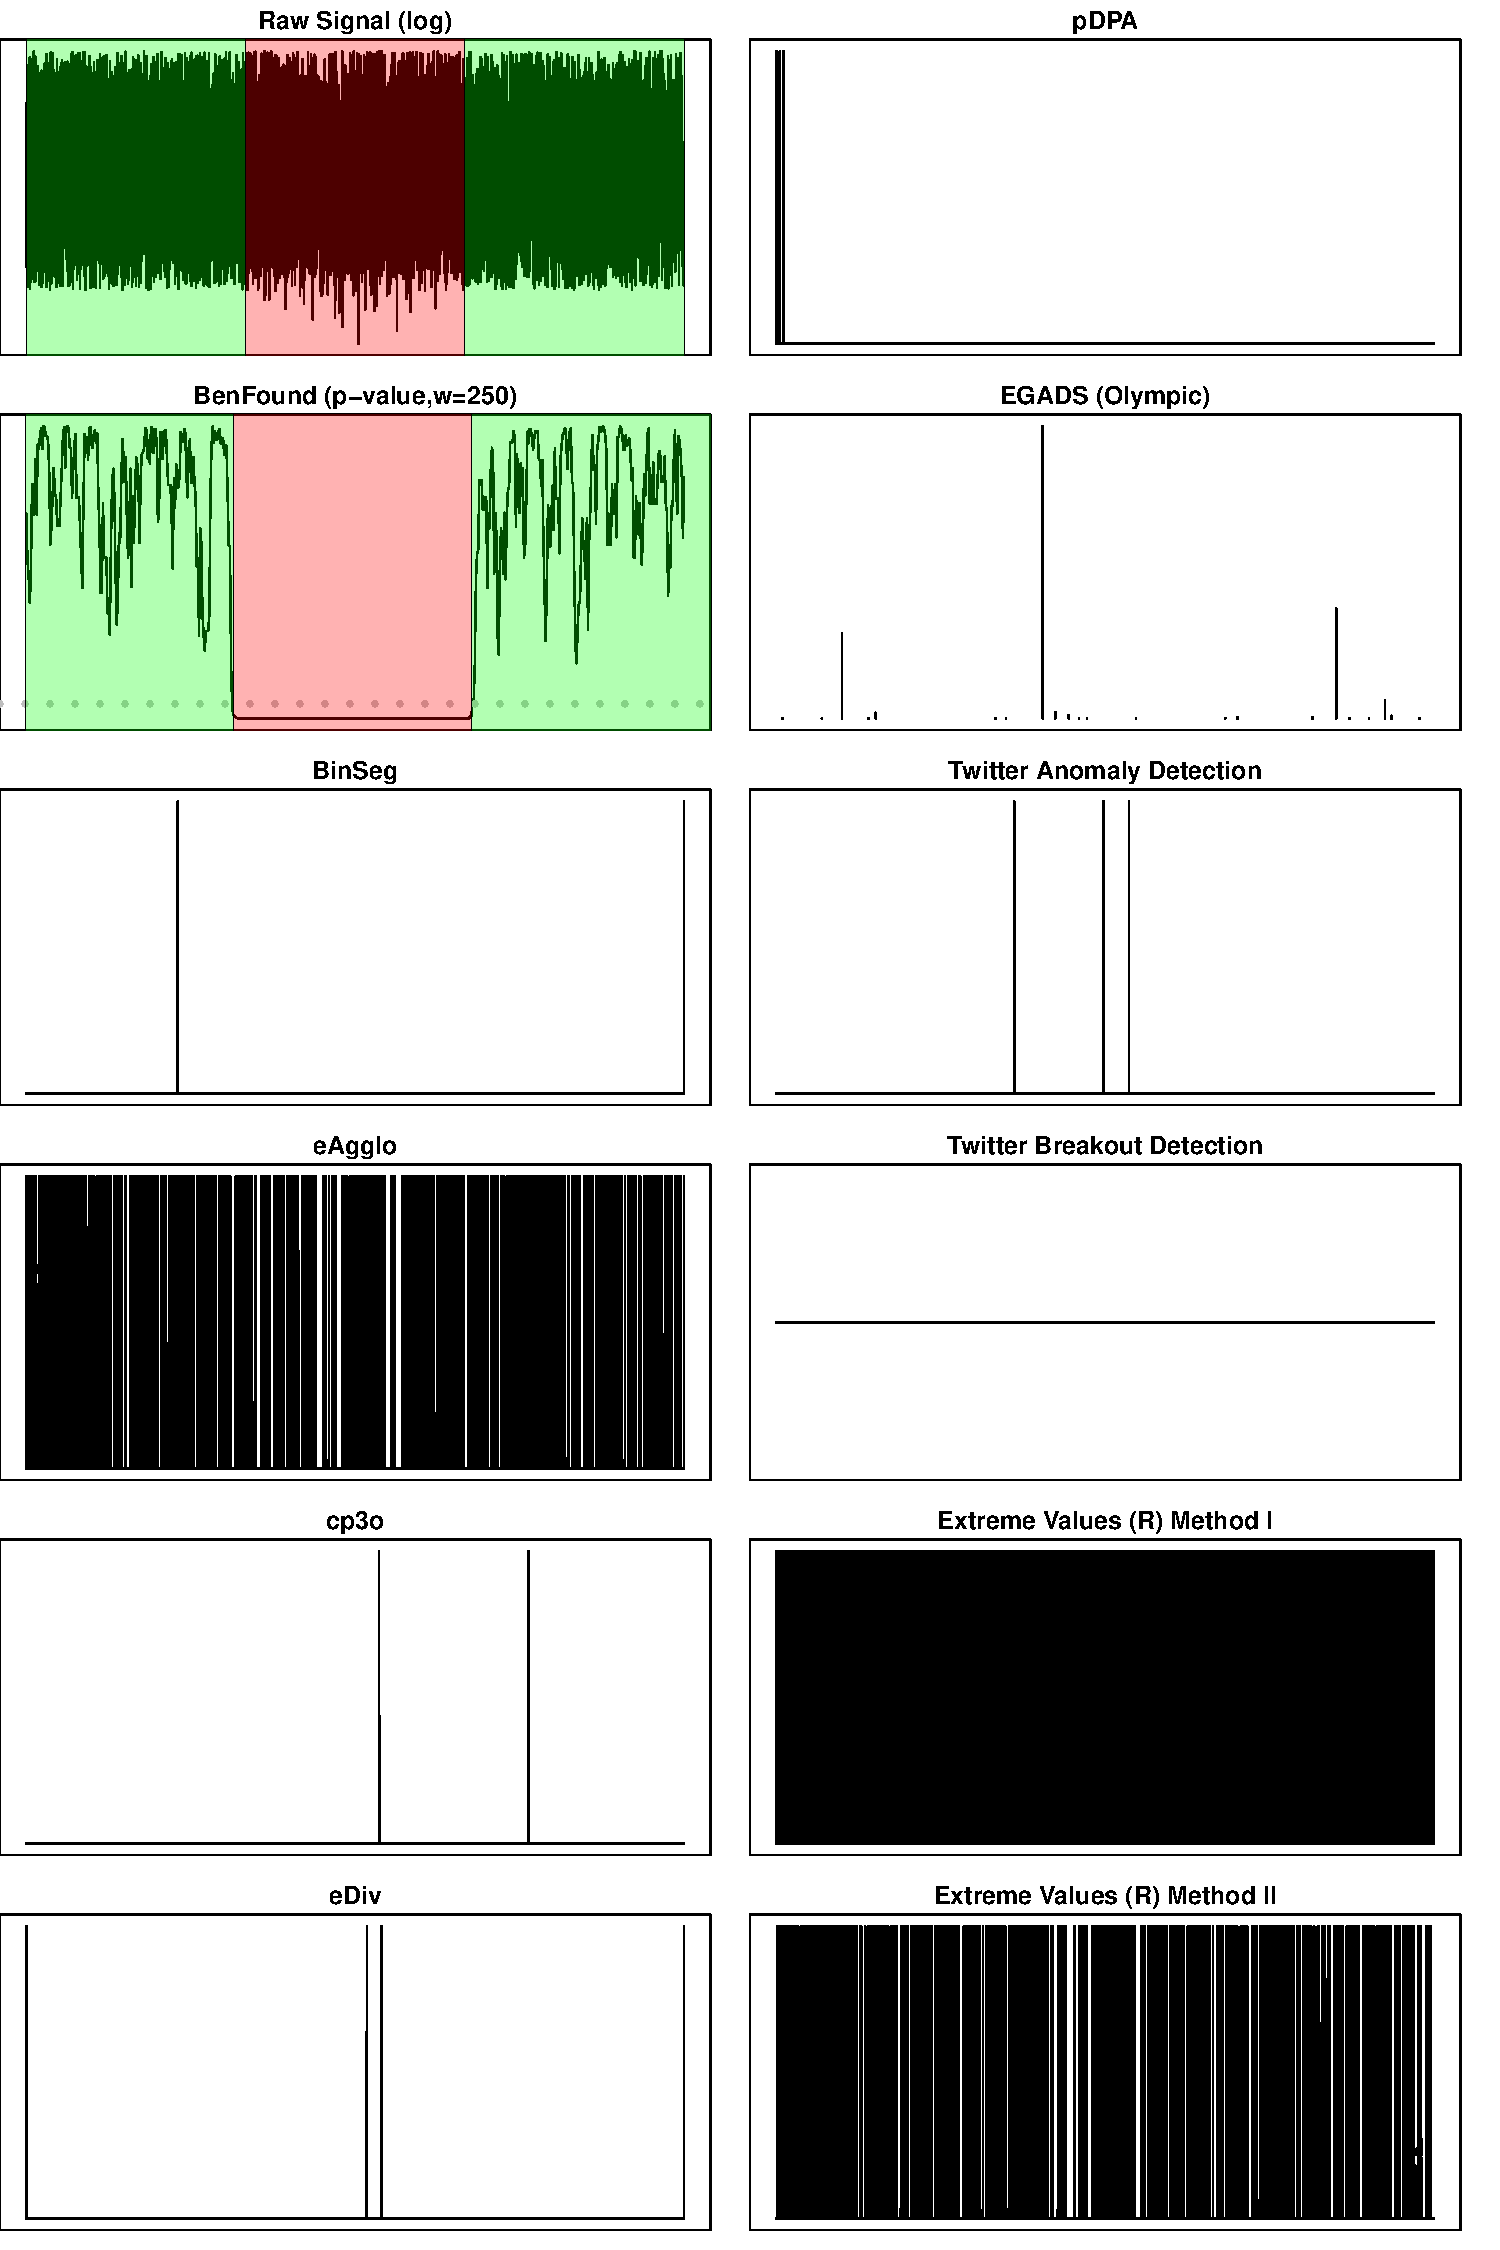
\includegraphics[width=\maxwidth]{figure/synthetic-experiments-1} \caption[A synthetically-generated time signal (top left) with Benford (green), non-Benford (red) and finally Benford (green) segments]{A synthetically-generated time signal (top left) with Benford (green), non-Benford (red) and finally Benford (green) segments. BenFound (row 2, col 1) is the only technique able to correctly detect the change in state and its regression.}\label{fig:synthetic-experiments}
\end{figure}


\end{knitrout}



%% Our real-world \textbf{#FathersDay} example showed, however, that the non-Benfordness in the \textit{lead-up} to Father's Day was explained by spammers hijacking the hashtag for advertising reasons. After Father's Day, the target for primarily ``organic'' tweets \textit{after} Father's Day.  

\section{Related Work and Discussion}
\label{sec:related-work}

BL was investigated in the context of online services for the first time in 2015 \cite{golbeck2015}. The primary contribution was to show that snapshots of randomly-sampled user metrics in \textit{social networks} (Facebook, Twitter, Pinterest) are Benford. The measurements in our introduction support this conclusion. In addition, we have presented results showing that metrics from Wikipedia, YouTube and GitHub are likewise Benford, and focused on the \textit{real-time} detection of BL \textit{deviations} in such systems.

A small set of dedicated BL reference volumes now exist. For theoretical and practical perspectives we respectively refer to \cite{berger2015Intro} and \cite{nigrini2012}. The latter focuses heavily on BL in forensic accounting, auditing and fraud detection. It treats BL-conformity tests and also compares BL to the well-known Zipf's Law, however it does not treat event-detection. In Section \ref{sec:test-conf-benf} we reevaluate the conformity tests and propose an alternative based on the formal Kolmogorov-Smirnov test.

The topics of event-, anomaly- and changepoint-detection have seen numerous contributions. Focusing firstly on Twitter-specific techniques, we find in \cite{ritter2012open} and \cite{hayashi2015real} two state-of-the-art approaches for the extraction of event phrases and topics from Twitter. Unlike \algoname{}, both rely on processing the tweet text stream. Additionally, whilst \algoname{} only raises a ``red flag'' when the digit distribution violates BL, these techniques \textit{continuously} yield a set of e.g. top-10 topics.

As \algoname{} is not restricted to text and graph structures, it is by no means restricted to social networks. \algoname{} can be applied to any numerical data stream obeying BL. In searching for comparison techniques we therefore extend our scope to the state-of-the-art in \textit{numerical} anomaly- and changepoint-detection from data-mining and statistics.

The most recent high-level contribution from the data-mining community is named the Extensible Generic Anomaly Detection System (EGADS in Figures \ref{fig:case-study-hashtag-hijacking-twitter} and \ref{fig:synthetic-experiments}) and stems from work at Yahoo \cite{laptev2015egads}. EGADS is a comprehensive framework that supports anomaly-detection based on a variety of configurable models, features and metrics. Two further approaches come from Twitter \cite{james2014twitter,vallis2014novel}. Twitter Anomaly Detection \cite{james2014twitter}, for example, employs time-series decomposition using statistical metrics to detect both global and local anomalies in the presence of seasonality and an underlying trend.

From the recent statistical literature we find in \cite{matteson2013} the non-parametric approach \eDiv{} that automatically detects both the number and location of change points. Unlike previous methods which typically focus on detecting a change in mean, variance or kurtosis, \eDiv{} is able to detect any distributional change. From the same work we find \eAgglo{}, the bottom-up variant of \eDiv{}, and another probabilistic pruning method \cpppo{}. These three methods are compared to \algoname{} in Figure \ref{fig:synthetic-experiments}. Each is designed for an offline setting and has a quadratic time complexity in the sample size $n$. %% Segments are found in a divisive hierarchical manner through the use of a binary bisection method. which merges segments such as to maximize a goodness-of-fit statistic.

The pruned dynamic programming algorithm \cite{rigaill2010} (\pDPA{} in Figure \ref{fig:synthetic-experiments}) is an offline approach which aims to infer both the number and positions of the change-points from the data. It uses a functional cost representation of segments in order to prune the search space of the segment neighborhood. It requires a user-specified parameter $k_{max}$ which represents the maximum number of change points to find. Its computational complexity is quadratic in the number of data points $n$.

Finally, we compare to Binary Segmentation \cite{scott1974Grouping,edwards1965cluster} (\BinSeg{} in Figure \ref{fig:synthetic-experiments}). This early approach detects changes in the mean and is commonly used as a baseline. 

                  %                   The approach aims to detect changes in a distribution's mean (\BinSegMean{}), variance (\BinSegVar{}) or both (\BinSegMeanVar{}). %%It exploits the hierarchical clustering technique of Edwards and Cavalli-Sforza \cite{edwards1965cluster} to split the time series into groups. 

                  %%                   The general problem concerns the inference of a \textit{change in the underlying distribution} that is responsible for generating a stream of time-ordered observations. Approaches to solving the problem can be divided into online and offline. In the online case, detection is done adaptively in real-time as new data arrives continuously. In the offline case, an entire history of time-ordered records is analyzed retrospectively. Approaches can further be characterized as parametric or non-parametric, and focus either on single or multiple changepoint detection. 


                  %%                   The Turbulence Time Series Event Detection and Classification (\TED{}) technique \cite{kang2014detecting} uses a two-step approach which extracts events from background fluctuations and groups dynamically-similar events into clusters. In contrast to the aforementioned methods which yield ``change-points'', \TED{} yields more precise ``events'' which encapsulate a start and end time. Like \algoname{}, \TED{} requires a user-specified sliding-window-size parameter.

Importantly, all of these approaches consider the distribution of the \textit{complete} numerical values in question. \algoname{}, in contrast, focuses on a particular kind of change event: a change in its leading digit distribution. This is achieved by considering BL and purposefully \textit{ignoring the magnitude information} of the temporal measurements. Fundamentally then, \algoname{} distances itself from the discussed state-of-the-art in that it does not look for changes to the underlying distribution of \textit{complete} values, but rather that of only the \textit{leading digits}. For this reason, \algoname{} has been able to correctly identify events in synthetic and real data (Sections \ref{sec:case-study:-twitter}, \ref{sec:case-study:-outag} and \ref{sec:synth-exper}) that are not found by any of the comparison techniques.

                  %                   In this way \algoname{} will not raise false alarms if measurements change magnitude but retain their ``natural'' digit distribution.

                  %                   If we focus on event detection in Twitter alone, a recent survey reviews a number of contributions \cite{atefeh2013Survey}. Five techniques are completely unsupervised, do not specify the type of event, and address the task of \textit{new} event detection. All five of these techniques, however, are dependent on the text stream and Twitter-specific features like Hashtags and retweet-counts.

                  %                   Zipf's law is a further empirical phenomenon that states that the frequency of utterances of any word in a natural language corpus is inversely proportional to its rank in the frequency table. Generally, data that conforms to BL does not conform to Zipf's Law and vice versa (\cite{nigrini2012}, Chapter 2). This is seen in a log-log plot of values versus ranks of our Twitter followers data\footnotemark[\ref{supMatFootnote}].

                  %                   <<zipf-plot,fig.width=10,fig.height=10,fig.pos='h',fig.cap='Log-log plot of value versus rank for our Twitter followers data.',echo=F,warning=F>>=

                  %                   ## Here we comment this out for space reasons. Uncomment this here and rebuild to see the plot.
                  %                   ## followersCountVectorOrdered <- followersCountVector[order(followersCountVector,decreasing=T)]
                  %                   ## plot(log(seq_along(followersCountVectorOrdered),base=10),log(followersCountVectorOrdered,base=10))
                  %                   @ 

Finally, our technique has \textbf{limitations}. Firstly, it is clearly only applicable to numeric data that obeys BL, meaning that it is inappropriate for many applications. Secondly, it requires a manual inspection step to analyze the cause for found events. Finally, it is not immune to false negatives. That is, if parties that artificially manipulate a system are aware of BL, they may tune their interactions such that the system metrics are not significantly affected from a BL perspective.

\section{Conclusion}

Various metrics from online services such as Twitter, Wikipedia, YouTube and GitHub naturally obey BL. When these metrics violate BL in real-time, it is often a sign of significant ``unnatural'' behavior. In this work we have proposed \algoname{}, a real-time event-detection approach for ``red-flagging'' such violations. In the case of online services, the interactions may be anti-social or malicious in nature, like non-permitted bot activity or hashtag-hijacking. We have compared \algoname{} to state-of-the-art event-detection techniques in controlled settings with synthetic data. Finally, we have deployed our technique to real-world settings and demonstrated practical knowledge discovery in various domains. \algoname{} is non-parametric, efficient and can be deployed in real-time on numerical data streams that obey BL.


\begin{thebibliography}{99}

\bibitem{alexander2009remarks}
  J.~Alexander, ``Remarks on the use of Benford’s Law'', 2009 (available at SSRN 1505147).

\bibitem{antoine2015portraying}
  {\'E}.~Antoine, A.~Jatowt, S.~Wakamiya, Y.~Kawai, and T.~Akiyama, ``Portraying collective spatial attention in twitter'', KDD 2015.

  
  
                  %                   \bibitem{atefeh2013Survey}
                  %                   F.~Atefeh, and W.~Khreich, ``A Survey of Techniques for Event Detection in Twitter'', in \emph{Computational Intelligence}, vol. 31, no. 1, 2015, pp. 132--164.
  
\bibitem{benford1938law}
  F.~Benford, ``The law of anomalous numbers'', in \emph{Proceedings of the American Philosophical Society}, vol. 78, 1938, pp. 551--572.

\bibitem{berger2011benford}
  A.~Berger, and T.P.~Hill. ``Benford’s Law strikes back: No simple explanation in sight'', in \emph{The Mathematical Intelligencer}, vol. 33, 2011, pp. 85--91.
  
\bibitem{berger2015Intro}
  A.~Nigrini, and T.P.~Hill, \emph{An Introduction to Benford's Law}. Princeton University Press, 2015.

\bibitem{edwards1965cluster}
  A.~Edwards and L.~Cavalli-Sforza, ``A Method for Cluster Analysis'', in \emph{Biometrics}, vol. 21, no. 2, 1965.
  
  %% \bibitem{kang2014detecting}
  %%   Y.~Kang, D.~Belu{\v{s}}i{\'c} and K.~Smith-Miles, ``Detecting and classifying events in noisy time series'', in \emph{Journal of the Atmospheric Sciences}, vol. 71, no. 3, 2014, pp. 1090--1104.

\bibitem{hayashi2015real}
  K.~Hayashi, T.~Maehara, M.~Toyoda and K.~Kawarabayashi, ``Real-time topic detection on twitter with topic hijack filtering'', KDD 2015.

\bibitem{james2014twitter}
  NA.~James, AK.~Kejariwal and DS.~Matteson, ``Leveraging Cloud Data to Mitigate User Experience
  from ‘Breaking Bad’'', arXiv preprint arXiv:1411.7955, 2014.
  
                  %                   \bibitem{killick2012optimal}
                  %                   R.~Killick, P.~Fearnhead and IA.~Eckley, ``Optimal detection of changepoints with a linear computational cost'',in \emph{Journal of the American Statistical Association}, vol. 107, no. 500, 2012, pp. 1590--1598.  
  
\bibitem{kolmogorov1933}
  A.~Kolmogorov. ``Sulla determinazione empirica di una legge di distribuzione''. Italian Actuarial Journal, 1933.

\bibitem{laptev2015egads}
  N.~Laptev, S.~Amizadeh, and I.~Flint, ``Generic and scalable framework for automated time-series anomaly detection'', KDD 2015.
  
\bibitem{matteson2013}
  D.~Matteson and N.~James. ``A Nonparametric Approach for Multiple Change Point Analysis of Multivariate Data'', in \emph{Journal of the American Statistical Association}, vol. 109, no. 505, 2014, pp.334-345.
  
\bibitem{nigrini2012}
  M.J.~Nigrini, \emph{Benford's Law: Applic. for Forensic Acc., Auditing and Fraud Det.}. John Wiley \& Sons, 2012.
  
                                                                                                        %                                                                                                         \bibitem{lemire2015}
                                                                                                        %                                                                                                         D.~Lemire, and L.~Boytsov. ``Decoding billions of integers per second through vectorization'', in \emph{Software: Practice and Experience}, vol. 45, 2015,pp. 1--29.
  
\bibitem{golbeck2015}
  J.~Golbeck. ``Benford's Law Applies to Online Social Networks'', in \emph{PloS one}, vol. 10, 2015.

\bibitem{rigaill2010}
  G.~Rigaill, ``Pruned Dynamic Programming for Optimal Multiple Change-Point Detection'', arXiv:1004.0887.
  
\bibitem{ritter2012open}
  A.~Ritter, Mausam, O.~Etzioni, S.~Clark, ``Open Domain Event Extraction from Twitter'', KDD 2012.

\bibitem{scott1974Grouping}
  A.~Scott and M.~Knott, ``A Cluster Analysis Method for Grouping Means in the Analysis of Variance'', in \emph{Biometrics}, vol. 30, no. 3, 1974, pp. 507--512.
  
\bibitem{twitterTos}
  Twitter Inc. ``Twitter Terms of Service''. Online Resource. https://www.twitter.com/tos.

\bibitem{vallis2014novel}
  O.~Vallis, J.~Hochenbaum and A.~Kejariwal, ``A novel technique for long-term anomaly detection in the cloud'', in 6th USENIX (HotCloud 2014).

  
\end{thebibliography}


\end{document}

                                                                                                        %                                                                                                         End of ltexpprt.tex
